
% !TEX root = NotesDeCours.tex



\part{Ecoulements compressibles}

% ================================================================================================ 
% Page de titre :
% ================================================================================================

\begin{frame}

  \color{bleu}

  \begin{flushleft}
    
    \Large
   	\bf
    
    Mécanique des fluides 

  \end{flushleft}
  
  \ligne{3} % remplace: \noindent \thickline{0.5mm}{150}

  \begin{flushright}

    \rm

    \textrm{David} \textsc{Fabre}
    
    \vspace{3mm}
    
    IMFT / UPS
    
    Département de Mécanique
    
  %  brancher@imft.fr

  \end{flushright}


\begin{picture}(105, 35)(0, 0)
  \put( 0,  0){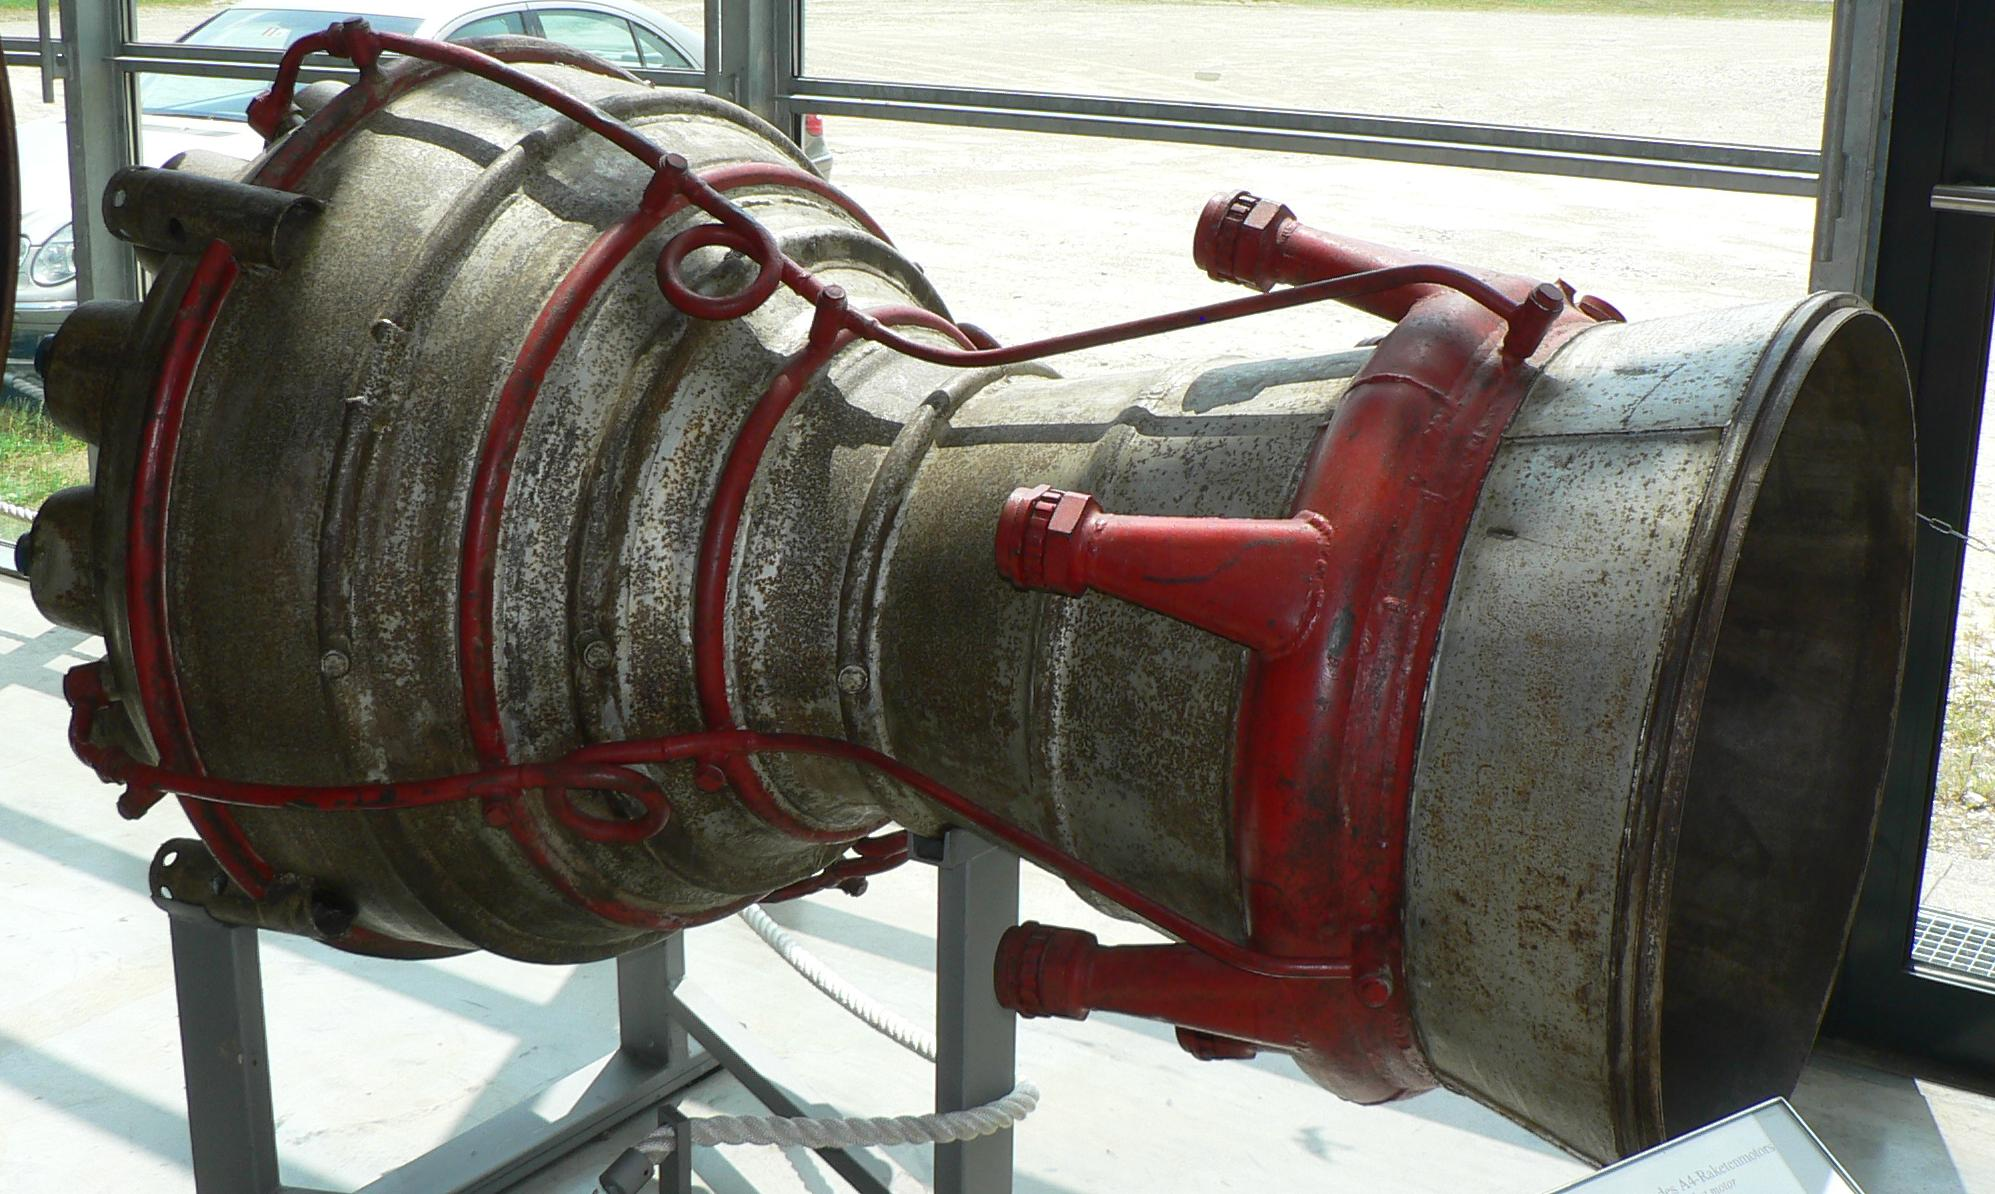
\includegraphics[height=40mm]{Rocket_nozzle_V2.jpg}}
  \put(69, 3){\color{gris} \small \rm \begin{minipage}{40mm}
  	Tuyère de fusée V2 de la \\
	seconde guerre mondiale.
	\end{minipage}}
\end{picture}

  \vspace{5mm}
  
  \begin{flushright}
    
    \Large
   	\bf
    
    
\quad  11. Ecoulements compressibles

  \end{flushright}

  \vspace{7mm}

\end{frame}

%%%%%%%%%%%%%%%%%%%%%%%%%%%%%%%%%%%%%%%%%%%%%%%%%%%%%%%%%%%%%%%%%%%%%%%%%%%%%%%%%%%%%%%%%%
% Sommaire :
%%%%%%%%%%%%%%%%%%%%%%%%%%%%%%%%%%%%%%%%%%%%%%%%%%%%%%%%%%%%%%%%%%%%%%%%%%%%%%%%%%%%%%%%%%
\handout{
\begin{frame}{Sommaire}

\small
  
\hspace*{2mm}
\begin{tabular}{cc}
		%&
  		\begin{minipage}{62mm}
  			\tableofcontents[firstsection=-9]
      \vspace{15mm}
  		\end{minipage}
  		&   
  		\begin{minipage}{60cm}
		  \vspace*{-5mm}  
  			%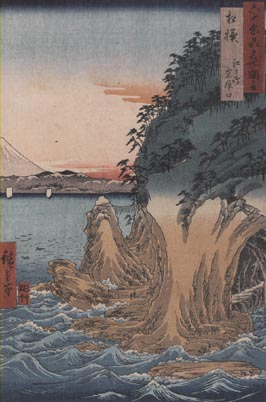
\includegraphics[width=40mm]{vagues.jpg} 
  		\end{minipage}
  	\end{tabular}

\vspace{0mm}

\end{frame}
}
%%%%%%%%%%%%%%%%%%%%%%%%%%%%%%%%%%%%%%%%%%%%%%%%%%%%%%%%%%%%%%%%%%%%%%%%%%%%%%%%%%%%%%%%%%
\section{\bfseries Ecoulements compressibles}
%%%%%%%%%%%%%%%%%%%%%%%%%%%%%%%%%%%%%%%%%%%%%%%%%%%%%%%%%%%%%%%%%%%%%%%%%%%%%%%%%%%%%%%%%%

%==========================================================================================
%\subsection{Introduction}
%=========================================================================================

\subsection{Equations du mouvement d'un gaz compressible}

\begin{frame}{Objectifs du chapitre et cadre d'étude}




\small

Objectifs du chapitre : 
\begin{itemize}
\item Introduire les équations régissant les écoulements {\em stationnnaires}  d'un gaz {\em compressible }.
\item Déterminer la forme optimale à donner à une tuyère de moteur-fusée pour optimiser la poussée.
\end{itemize}


\bigskip

\pause

Hypothèses de ce chapitre :  
\begin{itemize}
\item<1> Gaz parfait.
\item Ecoulement Inertiel ($Re \gg 1$) : frottement visqueux négligés 
\item Conduction thermique négligée ($Pe = \frac{U L}{\kappa} \gg 1$).
\item Pas de restriction sur le nombre de Mach ($M = {\cal O}(1) ) $.
\item Gravité négligeable.
\item Ecoulement stationnaire.  
\end{itemize}

\pause

\end{frame}

\subsubsection{Rappels de thermo et de cinétique des gaz}

%-----------------------------------------------------------------------------------------
\begin{frame}{Rappels : Description "milieu" continus d'un gaz parfait}

\small

Considérons un volume $V$ occupé par un nombre $N$ {\em très grand} de molécules (identiques) de masse individuelle $m_p$, de vitesses individuelles $\vec{v}_i$.

\pause 

{\em Ordre de grandeur : 
$N = {\cal O}({\cal N}_A)$ ; ${\cal N}_A = 6.22 \cdot 10^{26} $ nombre d'Avogadro.
}

\smallskip

%On définit $< \cdot > $ l'opérateur de moyenne statistiques. Celui-ci permet de définir successivement :

Le grand nombre de particules conduit à la nécessité d'un traitement statistique. On définit ainsi successivement :
\pause

\begin{itemize}

\item La densité volumique de particules $n^*$ (en particules/$m^3$) et la masse volumique $\rho$ 
(en $kg/m^3$ )
donnés par :
$$ n^* = \frac{N}{V} ; \quad \rho = n^* m_p = \frac{N m_p}{V} %= n M 
$$
\pause
%où $n = {\cal N}_A n^*$ est la densité volumique de moles de particules (en $mol/m^3$) 

%et $M ={\cal N}_A m_p $ la masse molaire (en $kg/mol$). 

\item La "vitesse moyenne de l'assemblée de particules" (ou vitesse au sens de la MMC) :
$$
\vec u = \left< \vec{v}_i \right> \equiv \frac{1}{N} \left(\sum\limits_{i=1}^N \vec{v}_i \right) 
$$
%(notation : $\left< f_i \right>  \frac{\sum\limits_{i=1}^n f_i }{N}$ est la moyenne statistique de la quantité définie à l'échelle microscopique $f_i$).
\pause
\item La vitesse quadratique moyenne $v_q$ :
$$
v_q^2 = \left< |\vec{v}_i-\vec{u}|^2 \right>   \equiv \frac{1}{N} \left(\sum\limits_{i=1}^N || \vec{v}_i-\vec{u}||^2  \right) 
$$
\pause
\item En invoquant le théorème de l'équipartition de l'énergie, cette dernière quantité permet de définir la température cinétique $T$ par :
$$
\frac{m_p v_q^2}{2} = 3 \frac{k_B T}{2} \qquad \mbox{ où } k_B = 1.38 \cdot 10^{-23}
\mbox{ est la constante de Boltzmann.}
$$
\pause 
$$\mbox{autre écriture :} \qquad v_q^2 = 3 r T \quad \mbox{ avec } r = \frac{k_b}{m_p} = \frac{R}{M}
$$
\end{itemize}

\end{frame}
 
\begin{frame}{Rappels : Lois d'état} 

\small 

\begin{itemize}

\item Loi d'état "mécanique" definissant la pression $p$

Celle-ci s'obtient en comptabilisant la force exercée sur une paroi due aux collisions.
\pause
\begin{itemize}

\item Expression microscopique : 
$$
\mbox{ } \quad 
p = \frac{N}{V} \frac{m_p v_q^2}{3} = \frac{N k_b T }{V }  
$$
 \pause
\item Expression macroscopique : 
$$ 
\mbox{ } \quad 
p = \rho r T \quad \left( \quad \mbox{ où }  r = \frac{k_B}{m_p} = \frac{R}{M} \right). 
$$

 où $R = {\cal N}_A k_B$ est la constante des gaz parfaits et $M ={\cal N}_A m_p $ la masse molaire. 
\end{itemize}
\pause
\item Loi d'état "énergétique" définissant l'énergie interne massique $e$ (ou une grandeur thermodynamique équivalente).
\begin{itemize}
\pause
\item 
Expression microscopique : Celle-ci s'obtient en comptabilisant les énergies élémentaires microscopiques 
 et en invoquant le théorème d'équipartition de l'énergie.

Pour un gaz parfait diatomique {\color{gray} (5 ddl par particule, 3 translations + 2 rotations)} :
$$
e = \frac{1}{N m_p} \times 5 N  \times \frac{k_B T}{2} = \frac{5 r T}{2} \quad \left( \equiv \frac{5}{3} v_q^2 \right)
$$

\pause
\item %Deuxième forme faisant intervenir l'enthalpie massique $h = e + p/\rho$ : 
Expression macroscopique : 
$$ e = c_v T \quad \mbox{  avec } c_v = \frac{5 r}{2} ; \qquad  
h = e+ \frac{p}{\rho} = c_p T \quad \mbox{  avec } c_p= c_v + r = \frac{7 r}{2} 
$$
%$$
%h = e + r T = \frac{7 r T}{2}
%\quad \left( \equiv \frac{7}{3} v_q^2 \right)
%$$
\pause

\item Généralisation : pour un gaz défini par son indice adiabatique $\gamma = c_p / c_v$ :
$$
e = c_v T \mbox{ avec } c_v = \frac{\gamma r }{\gamma -1} ; \qquad 
h = c_p T \mbox{ avec } c_p = \frac{ r }{\gamma -1}   \quad \left( \gamma = \frac{c_p}{c_v} \right)
$$
\end{itemize}



 \end{itemize}
\end{frame}



\begin{frame}{Rappels : Compressibilité et vitesse du son} 

\small 

A partir des lois d'état on définit le coefficient de compressibilité :
$$
\chi_S = \frac{1}{\rho} \left(\frac{\partial \rho}{\partial p}\right)_{s}
$$
\pause

Celui-ci permet de définir une échelle de vitesse caractéristique : la {\em vitesse du son} 
$$
c^2 =  \left(\frac{\partial p}{\partial \rho}\right)_{s} = \frac{1}{\rho \chi_S}
$$

\pause
Pour un gaz parfait : $c^2 = \gamma p/\rho = \gamma r T$ 

\pause
\begin{itemize}
\item Lien avec la vitesse quadratique moyenne :
$$
c^2 = \frac{\gamma}{3} v_q^2
$$ 
\pause
\item Lien avec l'énergie massique et l'enthalpie massique :
$$
c^2 = \frac{\gamma e }{\gamma -1} 
$$

$$
c^2 = \frac{ h }{\gamma -1} 
$$



 \end{itemize}



 \end{frame}
 

%-----------------------------------------------------------------------------------------
\subsubsection{Rappels : Nombre de Mach}
%-----------------------------------------------------------------------------------------
\begin{frame}{Rappels : Nombre de Mach}
%-----------------------------------------------------------------------------------------

\small

On appelle \textcolor{vert}{nombre de MACH} le rapport sans dimension
\[
	\color{red}
	M = \frac{u}{c}
\]
où $u$ désigne la vitesse locale de l'écoulement %.et
%\[
%	\color{blue}
%	c^2 = \dfrac{1}{\rho \kappa_s} = \left ( \dfrac{\partial p}{\partial \rho}\right )_{s}
%\]
%correspond au carré de la vitesse locale du son.

\medskip
\pause

%De l'isentropie ($ds=0$) 
%Pour un gaz parfait, on déduit :
%$
%	c^2 = \dfrac{\gamma p}{\rho} = \gamma r T = \frac{h}{\gamma-1} 
%$

\bigskip
\pause

La valeur du nombre de Mach définit le type d'écoulement rencontré :

\smallskip

\begin{itemize}
\item
	$0 < M <1$ : écoulement \textcolor{vert}{subsonique} (vitesse de l'écoulement $<$ vitesse du son)
\item
	$M \rightarrow 0$ : écoulement \textcolor{vert}{incompressible}
\item
	$M \approx 1$ : écoulement \textcolor{vert}{transonique}
\item
	$M=1$ : écoulement \textcolor{vert}{sonique}
\item
	$M > 1$ : écoulement \textcolor{vert}{supersonique} (vitesse de l'écoulement $>$ vitesse du son)
\item
	$M \gg 1$ : écoulement \textcolor{vert}{hypersonique}
\end{itemize}

\vspace{0mm}

\end{frame}



%------------


\subsubsection{Equations d'Euler compressible}

\begin{frame}{Equations du mouvement pour un gaz compressible}
\small

Rappel des hypothèses :  
\begin{itemize}
\item Gaz parfait.
\item Ecoulement Inertiel ($Re \gg 1$) : frottement visqueux négligés 
\item Conduction thermique négligée ($Pe = \frac{U L}{\kappa} \gg 1$).
\item Pas de restriction sur le nombre de Mach ($M = {\cal O}(1) ) $.
\item Gravité négligeable.
\item Ecoulement stationnaire.  
\end{itemize}

\pause 
\medskip 

Sous ces hypothèses les équations de la masse et de la quantité de mouvement sont 
les équations d'Euler compressibles stationnaires :

$$
\divergence ( \rho \vec{u} ) = \rho \divergence ( \vec{u} ) + \vec{u} \cdot \gradient (\rho) = 0.
$$
$$
\rho  \left[ \mytensor{grad}\left( \vec{u} \right) \cdot \vec{u}\right]  = - \gradient (p)
$$

\pause
Questions :
\medskip

\pause

Peut-on utiliser Bernoulli pour relier $p$ et $u = |\vec{u}|$ ? 

\pause 

$=>$ Non ! 
\medskip

\pause
Peut-on pour autant trouver une relation générale reliant $u$ et $p$ (ou une autre quantité thermodynamique) le long de chaque ligne de courant ?

\pause
$=>$ Il faut travailler a partir du {\em bilan d'énergie totale} au lieu du bilan d'energie cinétique....

\end{frame}

\subsubsection{Equation-bilan de l'énergie totale}

\begin{frame}{Bilan d'énergie totale (1er principe)}
\small

Ecrivons un bilan d'énergie (premier principe) pour un volume {\em de contrôle} $\Omega$ (cf. formulaire, annexe B.4)

\begin{equation}
		\underbrace{\dpdt{} \int_{\Omega} \rho \left( e + \frac{ |\vec{u}|^2}{2} \right) \; dV
		}_{\ddt{E_{\Omega}} }		 
		= \underbrace{  - \oint_{\partial \Omega}  \rho \left( e + \frac{ |\vec{u}|^2}{2} \right) \vec{u} \cdot \vec{n} \; dS
		}_{\dot{E}^{(ech)}}
	%	+ \underbrace{\int_{\Omega} \rho \vec{f} \cdot \vec{u} \; dV
	%	}_{\dot{W}^{(f)}} 
		+ \underbrace{ \oint_{\partial \Omega} -p \vec{u} \cdot  \vec{n}   \; dS 
		}_{\dot{W}^{(p)}} 
	%	+ \underbrace{ \oint_{\partial \Omega} \vec{u} \cdot  \mytensor{\tau} \cdot \vec{n}  \; dS 
	%	}_{\dot{W}^{(v)}} 
	%	 \underbrace{ - \oint_{\partial \Omega} \vec{q} \cdot \vec{n} \; dS
	%	}_{\dot{Q}} 
		\label{eq:bilan_global_eulerien_e1}
\end{equation}

{\color{gris}{\tiny Remarques : 

$\dot{Q} = 0$ car on néglige les échanges de chaleur (adiabatique) ; 

$\dot{W}^{(p)} \equiv -P dV/dt$ si $p$ est uniforme ($p\equiv P$) ; 

On retrouve alors dans ce cas l'expression classique du travail de pression du cours de thermodynamique}}

\smallskip
\pause

En régime stationnaire, ce bilan devient :
\begin{equation}
 \oint_{\partial \Omega}  \rho \left( h + \frac{ |\vec{u}|^2}{2} \right) \vec{u} \cdot \vec{n} \; dS
=0		
\label{eq:bilan_global_eulerien_e2}
\end{equation}

\pause

Ce qui, a l'aide du théorème de la divergence et en utilisant l'équation-bilan de masse 
conduit à un bilan local sous la forme :
$$ 
%\rho \frac{ d }{dt}  \left( h + \frac{|\vec{u}|^2}{2} \right) =
\rho \vec{u} \cdot \gradient \left( h + \frac{|\vec{u}|^2}{2} \right) = 0. 
$$

\medskip
\pause

Conclusion : l'enthalpie totale massique ${\cal H} = h + \frac{|\vec{u}|^2}{2}$ est conservée le long de chaque ligne de courant.

%On peut aussi introduire l'\textcolor{vert}{enthalpie totale} moyenne, somme de l'énergie "thermodynamique" 
%(enthalpie spécifique) et de l'énergie cinétique :
%\[
%	\color{vert}
%	{\cal H} \equiv h + \frac{1}{2} u^2 = e + \frac{p}{\rho} + \frac{1}{2} u^2 = c_p \, T + \frac{1}{2} u^2
%\]
%\pause
%Le bilan pour l'enthalpie totale s'écrit alors :
%\[
%	\color{red}
%  d{\cal H}  = 0 \quad \Leftrightarrow \quad {\cal H} = Cte
%\]



\end{frame}


\begin{frame}{Conditions génératrices} 

\small

Définition : {\bf  Conditions génératrices} 

Supposons que toutes les lignes de courant proviennent d'une région  {\em de stagnation} 
où la vitesse est nulle ($u=0$) et où les variables thermodynamiques ont pour valeur les  "conditions génératrices"  $,p_i ; \rho_i ; T_i, h_i ; c_i$. 
\smallskip
\pause

Alors la conservation de l'enthalpie totale peut se mettre sous les formes équivalentes suivantes :
\pause
\medskip
\begin{itemize}

\item $ h + \frac{u^2}{2} = h_i$ 

$h_i$ est l'enthalpie génératrice (enthalpie d'un "point d'arrêt" de l'écoulement où $u=0$).
\pause
\item $c_p T + \frac{u^2}{2} = C_p T_i$

 $T_i$ est la température génératrice.
\pause
\item $\frac{c^2}{\gamma-1} + \frac{u^2}{2}  = \frac{c_i^2}{\gamma-1}$

$c_i = \sqrt{\gamma r T_i}$ est la vitesse du son correspondant aux conditions génératrices.
\pause
\item $\frac{T}{T_i} = \frac{c^2}{c_i^2} = \left( 1 + \frac{\gamma-1}{2} M^2 \right)^{-1}$

Cette dernière forme est appelée {\bf 1ère relation de Barré de St Venant}. 

\end{itemize}

%\pause
%\bigskip
%Application : "tube de pitot thermique" permettant de mesurer (théoriquement) $u$ a partir de $T_i$ et $T$.

%{\textcolor{gris} (en pratique difficile à mettre en oeuvre car il faudrait un matériau non conducteur de la chaleur).}


\end{frame}

%\subsubsection{Bilan d'entropie}
%
%\begin{frame}{Bilan d'entropie}
%
%\small
%Sous les hypothèses de ce chapitre formulées plus haut, on a négligé tous les phénomènes dissipatifs (irréversibles), a savoir le {\em frottement visqueux} et la {\em conduction thermique}.
%
%\medskip
%\pause 
%
%Le bilan local d'entropie est donc :
%
%
%\medskip 
%$$
%%\mbox{ forme locale : } 
%\rho \frac{ds}{dt} =  \rho \vec{u} \cdot \gradient (s) = 0.
%$$
%
%(démo plus rigoureuse, cf. annexe A.6).
%\pause
%\bigskip
%
%$=>$ L'entropie massique $s$ se conserve le long des lignes de courant.
%
%\pause
%\medskip
%Sur les lignes de courant on pourra donc utiliser les relations de Laplace :
%
%%En effet, on peut vérifier que l'écoulement est isentropique :
%\[
%%	\mbox{\color{gris} [Démonstration] \; $\longrightarrow$ \;}
%	\color{red} 
%	T\rho^{1-\gamma} = Cte \quad \mbox{\color{black} et} \quad p\rho^{-\gamma} = Cte
%\]
%
%
%
%\end{frame}

\subsubsection{Relations de Barré--St Venant}

%-----------------------------------------------------------------------------------------
\begin{frame}{Relations de Barré--St Venant}
%-----------------------------------------------------------------------------------------

\small

En supposant qu'on peut négliger les phénomènes dissipatifs (viscosité et conduction thermique) l'écoulement est {\em isentropique}.
\pause

Les {\bf relations de Laplace}  permettent alors de déterminer les conditions de l'écoulement en tout point en fonction du nombre de Mach local et des conditions génératrices.

\medskip
Ce sont les {\bf Relations de Barré de St-Venant :}

\begin{color}{red} 
\begin{eqnarray*}
	\mbox{\color{gris} [Démonstration] \; $\longrightarrow$ \;}
	\color{red}\frac{T}{T_i} & = & \left ( 1 + \frac{\gamma-1}{2} M^2 \right )^{-1}	;
	\quad
	\color{red} \frac{\rho}{\rho_i}  \; =  \; \left ( 1 + \frac{\gamma-1}{2} M^2 \right )^{\dfrac{1}{1-\gamma}}	
	\\
	\color{red} \frac{p}{p_i} & = & \left ( 1 + \frac{\gamma-1}{2} M^2 \right )^{\dfrac{\gamma}{1-\gamma}} ; \quad 
	%\\
	\color{red} u  =  M \sqrt{\gamma r T_i} \left ( 1 + \frac{\gamma-1}{2} M^2 \right )^{-1/2}
\end{eqnarray*}
\end{color}

\medskip \pause

\textbf{Remarques :} \medskip

tous les rapports $T/T_i$, $\rho/\rho_i$ et $p/p_i$ sont \\
des fonctions décroissantes du nombre de Mach $M$. 

\medskip

$u$ est par contre une fonction croissante du nombre \\
de Mach $M$.

\begin{picture}(0, 0)(-60, 8)
	\put(0, 0){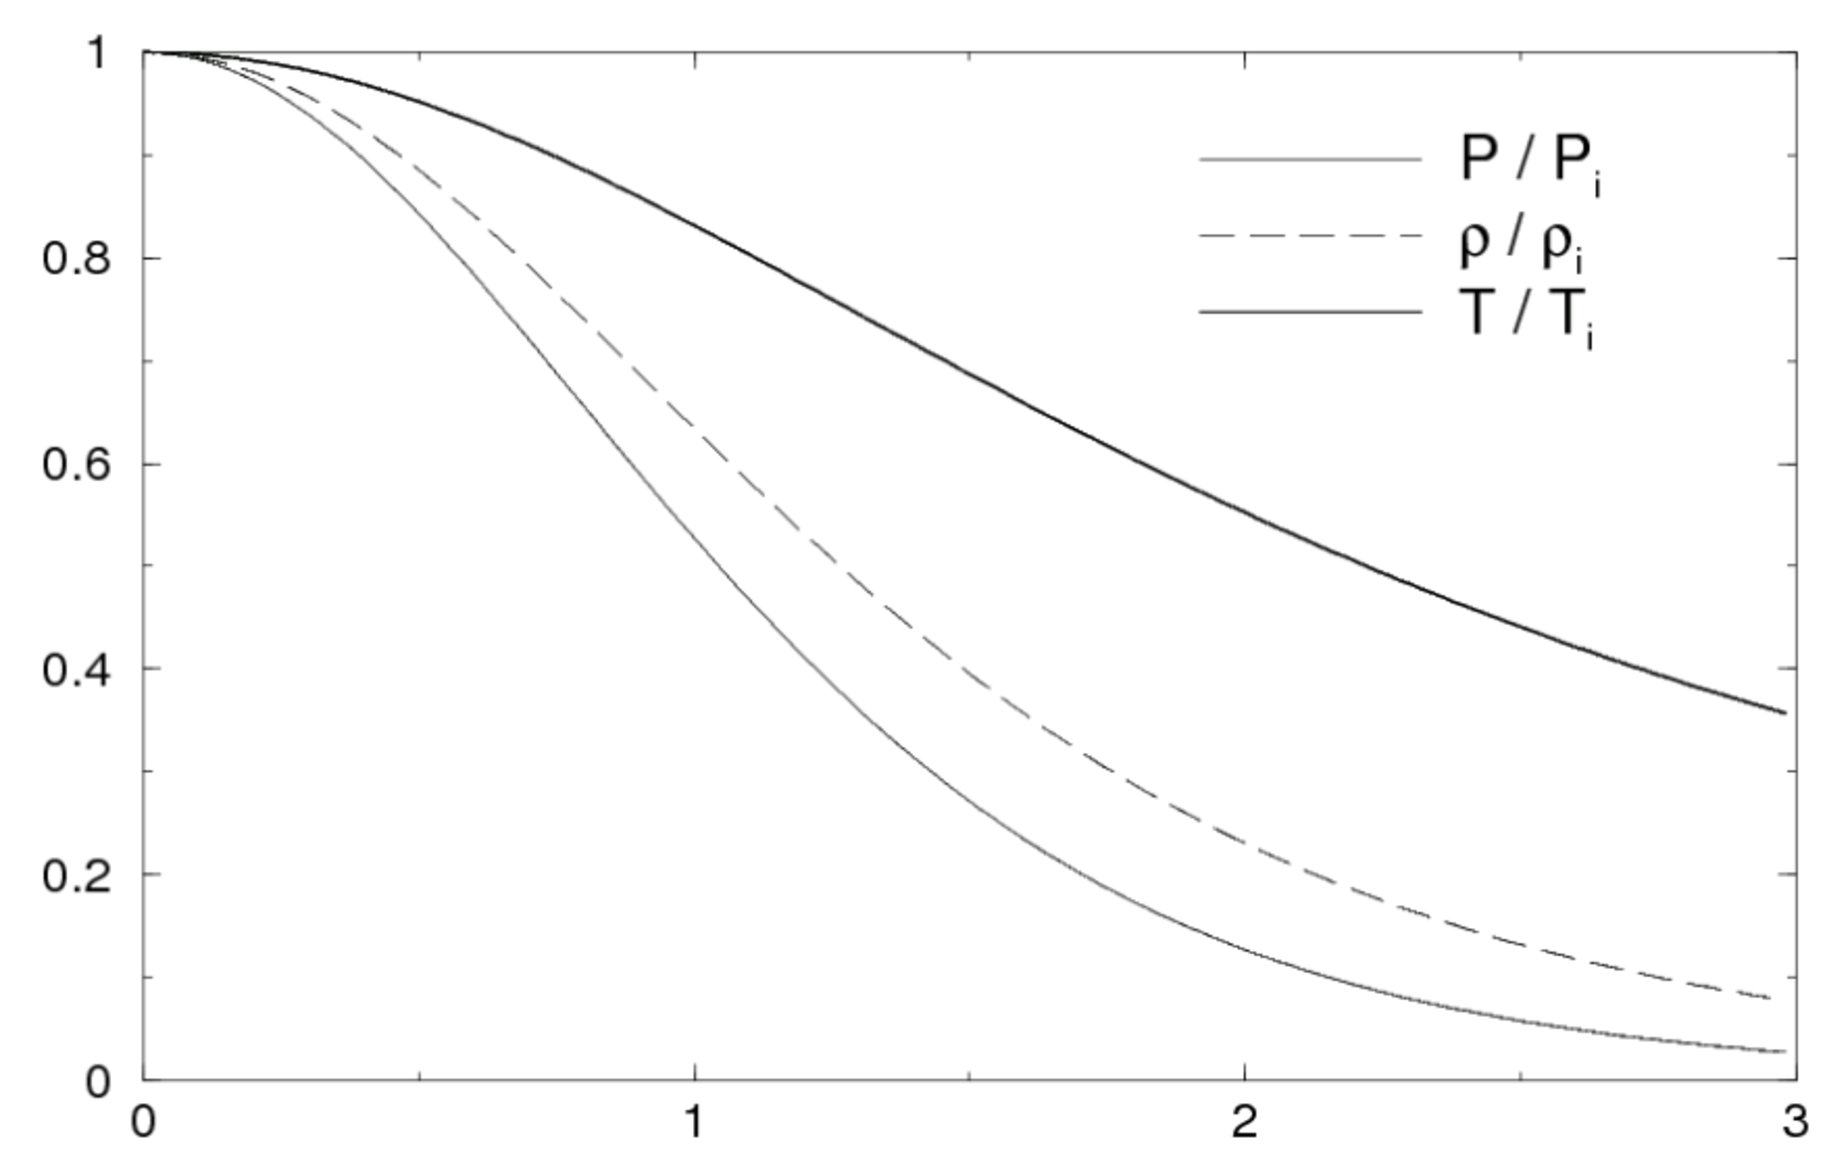
\includegraphics[width=45mm]{saint_venant.pdf}}
	\put(22, -1){\footnotesize $M$}
	\put(29, 23){\colorbox{white}{\color{white}\scriptsize $p/p_i$ $p/p_i$}}
	\put(29, 20){\colorbox{white}{\color{white}\scriptsize $p/p_i$ $p/p_i$}}
	\put(16, 9){\footnotesize $p/p_i$}
	\put(24, 13){\footnotesize $\rho/\rho_i$}
	\put(30, 17){\footnotesize $T/T_i$}
\end{picture}

\vspace{1cm}

\pause 

\textbf{Exercice :} \medskip
Montrez que dans la limite $M \ll 1$ les troisième et quatrième relations permettent de retrouver le 1er théorème de Bernoulli : \quad
$\displaystyle p + \rho_i \frac{u^2}{2} = p_i +o(M^2) $


\vspace{10mm}

\end{frame}


%-----------------------------------------------------------------------------------------
\subsection{Ecoulements compressibles monodimensionnels isentropiques}
\subsubsection{Objectifs et hypothèses de modélisation}

%-----------------------------------------------------------------------------------------
\begin{frame}{Ecoulements compressibles monodimensionnels : Objectifs}
%-----------------------------------------------------------------------------------------

\small


%\item<1->
%	Prise en compte des effets de compressibilité du fluide en écoulement.
%\item<2->%
%	Application aux écoulements en conduite, en particulier 
%	pour justifier la séquence
%	\\ \medskip
%	\centerline{\color{red} convergent $\rightarrow$ col $\rightarrow$ divergent} 
%	\smallskip
%	employée pour les tuyères pour maximiser la poussée du réacteur %$\color{red} F = \dot{m}U = \rho U^2 A_s$
%	\\
%	où $A_s$ désigne la section de sortie du réacteur, et $U$ la vitesse en sortie.
%	\\ 
%	\medskip
%	\begin{picture}(80, 35)(0, 0)
%		\put(0, 0){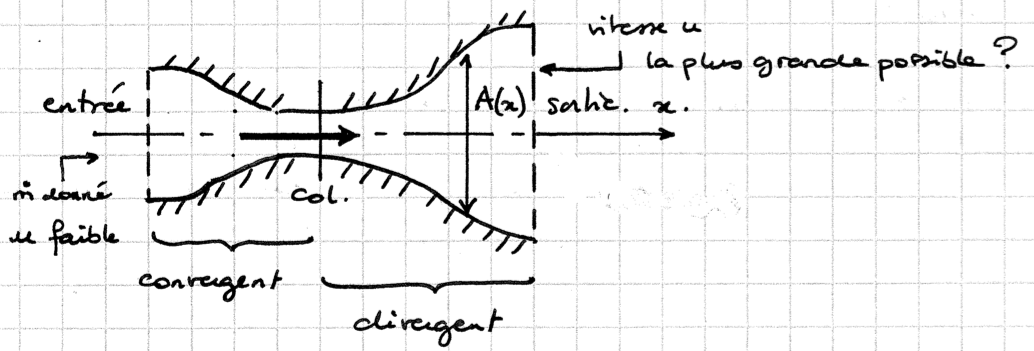
\includegraphics[width = 90mm]{tuyere.png}}
%	\end{picture}

Application : considérons maintenant le cas d'un moteur-fusée, alimenté par un réservoir de grande dimension
dans lequel le gaz est dans  les conditions génératrices,
reliée à une tuyère  dont la forme présente un conduit {\bf convergent}, suivi d'un {\bf col  } puis d'un conduit {\bf divergent}.


\begin{center}
	\begin{picture}(70, 25)(0, 0)
		\put(0, 0){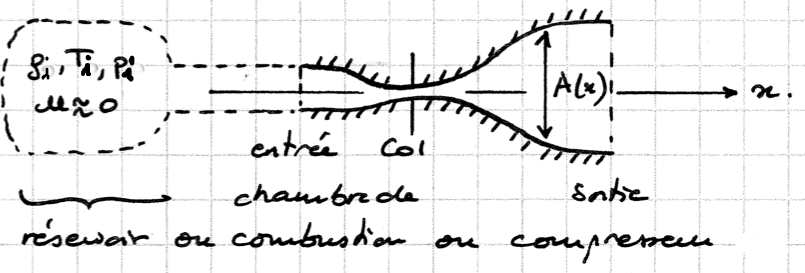
\includegraphics[width = 70mm]{conditions_generatrices.png}}
	\end{picture}
\end{center}


	
	\medskip
%\item[\checkmark]<3->
%	Mise en équation : modélisation dans le cadre de l'\textcolor{vert}{approximation unidimensionnelle}

Aux hypothèses générales du chapitre on rajoute la suivante : 

\begin{itemize}
	\item[\checkmark] {\bf Ecoulement monodimensionnel : }
	$\color{vert} \myvec{u}(x, y, z, t) \approx u(x)\, \myvec{e}_x$ \quad$\; \color{vert} \rho(x, y, z, t) \approx \rho(x),
\quad p(x, y, z, t) \approx p(x), \quad T(x, y, z, t) \approx T(x), \ldots$
	
	(valide si les variations de section sont faibles ; $\partial A/ \partial x \ll 1$).
	
	%\item[\checkmark] {\bf Ecoulement isentropique }
	
	%(valide si les mécanismes de diffusion sont négligeagles)


\item Objectif : déterminer $u,p,\rho,T...$ en tout point $x$ de la tuyère.

Grâce aux relations de St Venant il suffit de savoir calculer $M$ en fonction de $x$ (ou plutôt en fonction de $A$).


\item Dans un premier temps établissons une relation très importante entre les variation de vitesses $du$ et de section $dA$


\end{itemize}



\vspace{5mm}

\end{frame}

%-----------------------------------------------------------------------------------------

%-----------------------------------------------------------------------------------------

%%-----------------------------------------------------------------------------------------
%\begin{frame}{Modélisation : approximation unidimensionnelle (1D)}
%%-----------------------------------------------------------------------------------------
%
%\small
%On considère l'écoulement dans un tube de courant donné, d'axe $\myvec{e}_x$,
%par exemple les parois \\ d'une conduite de section variable $A(x)$.
%
%\smallskip
%
%Si les variations de section $A(x)$ ne sont pas trop fortes, alors il est raisonnable
%d'approximer \\
%les grandeurs physiques $F$ par leur valeur moyenne dans chaque section $A(x)$ :
%\[
%	\color{red}
%	F(x, y, z, t) \sim \overline{F}(x, t)
%\] 
%avec \;
%$ \displaystyle
%  \color{vert}
%  \overline{F}(x, t) \equiv \frac{1}{A(x)} \int_{A(x)} F(x, y, z, t) \, dS
%  \pause
%  \color{black}
%  \; \Leftrightarrow \; 
%  \int_{A(x)} F(x, y, z, t) \, dS  = A(x) \, \overline{F}(x, t)
%$
%
%\bigskip
%\pause
%
%\textbf{Domaine de validité :}
%
%\begin{equation*}
%	F(x, y, z, t) = \overline{F}(x, t) + F'(x, y, z, t) \approx \overline{F}(x, t)
%	\quad \mbox{si} \quad
%	\left | \frac{F'}{\overline{F}}\right | = \mathcal{O}(\varepsilon) \ll 1
%\end{equation*}
%
%\medskip
%\pause
%\textbf{Remarques :} 
%
%\medskip
%
%La moyenne des fluctuations est nulle :
%\[
%	\mbox{\color{gris} [Démonstration] \; $\longrightarrow$ \;}
%	\color{red}
%	\overline{F'}(x, t) = 0
%\]
%
%\pause
%\smallskip
%
%A l'ordre $\mathcal{O}(\varepsilon)$, si $F_1$ et $F_2$ sont deux grandeurs physiques quelconques, alors
%
%\[
%	\mbox{\color{gris} [Démonstration] \; $\longrightarrow$ \;}
%	\color{red}
%	\overline{F_1F_2}(x, t) \approx \overline{F_1}(x, t) \times \overline{F_2}(x, t)
%\]
%
%
%\vspace{0mm}
%
%\end{frame}

%%-----------------------------------------------------------------------------------------
%\begin{frame}{Modélisation : cadre}
%%-----------------------------------------------------------------------------------------
%
%\small
%
%\textbf{Hypothèses de travail :} \pause
%Aux hypothèses générales de ce chapitre :  
%\begin{itemize}
%\item Gaz parfait.
%\item Ecoulement Inertiel ($Re \gg 1$) : frottement visqueux négligés 
%\item Conduction thermique négligée ($Pe = \frac{ U L}{k} \gg 1$).
%\item Pas de restriction sur le nombre de Mach ($M = {\cal O}(1) ) $.
%\item Gravité négligeable.
%\item Ecoulement stationnaire.  
%\end{itemize}
%	
%\smallskip
%	
%On rajoute l'hypothèse supplémentaire
%\begin{itemize}
%	\item[\checkmark] Ecoulement monodimensionnel : 
%	
%	$\color{vert} \myvec{u}(x, y, z, t) \approx u(x)\, \myvec{e}_x$ \quad
%$\; \color{vert} \rho(x, y, z, t) \approx \rho(x),
%\quad p(x, y, z, t) \approx p(x),
%\quad T(x, y, z, t) \approx T(x), \ldots$
%	
%	
%\end{itemize}	
%
%
%\vspace{15mm}
%
%\end{frame}

%\subsubsection{Bilan de masse}

%==========================================================================================
\subsubsection{Equations-bilan et Relation de Hugoniot}
%=========================================================================================

%-----------------------------------------------------------------------------------------
\begin{frame}{Equations-bilans sous l'hypothèse monodimensionnelle : principe}
%-----------------------------------------------------------------------------------------

\small

On a besoin d'écrire les équations-bilan de masse,  énergie totale et entropie :

\begin{itemize}

\item Sur une section de conduite d'aire d'entrée $A_1$ et d'aire de sortie $A_2$ ;

\begin{center}

	\begin{picture}(53, 22)
	\scriptsize
		\put(0, 0){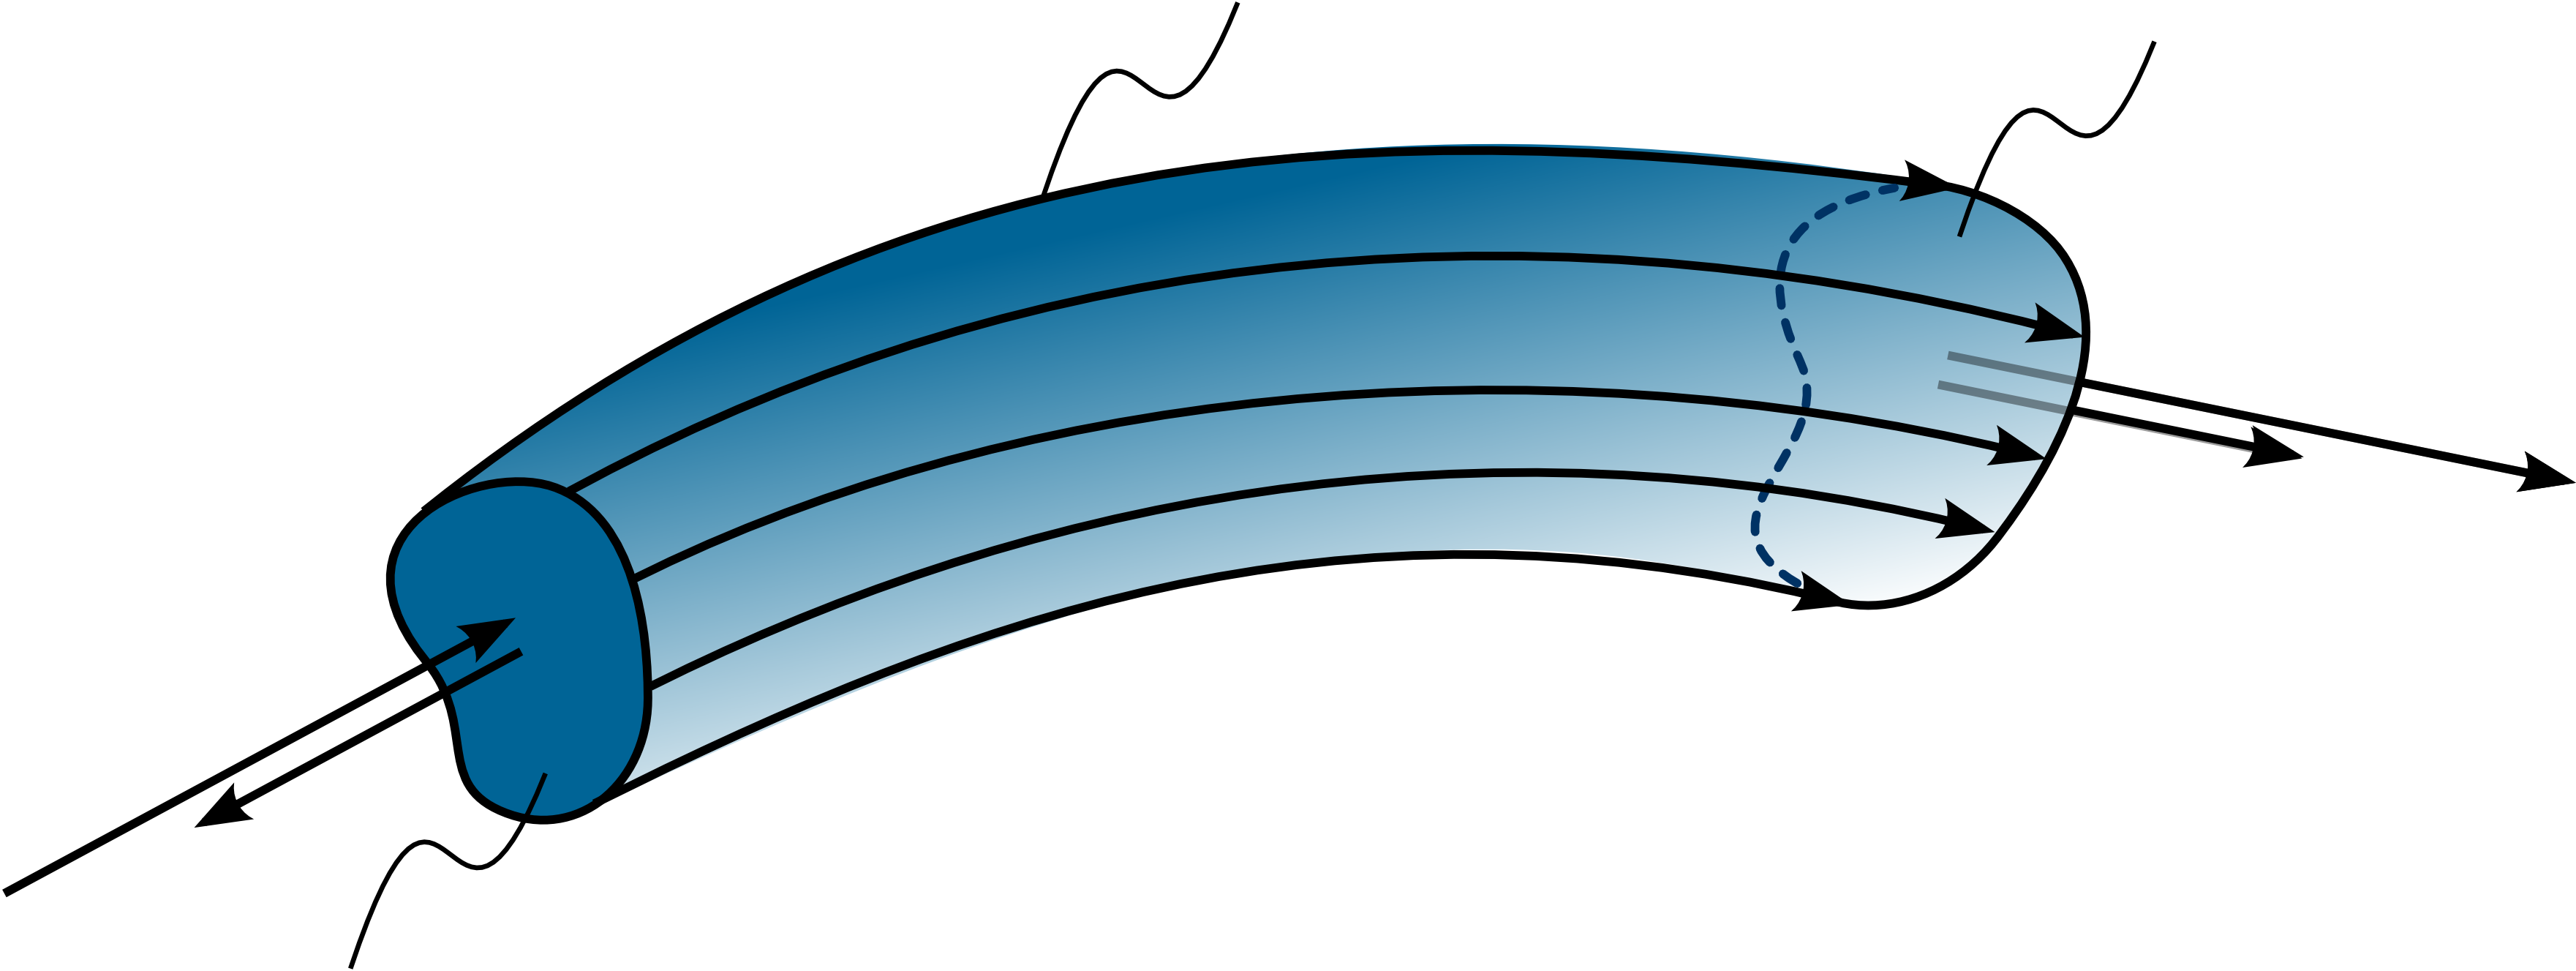
\includegraphics[width=53mm]{streamtube.png}}
		\put(5.3, -2){$\Gamma_1$ (entrée)}
		\put(3, .7){$\myvec{n}_1$}
		\put(-4, 8.3){$P_1,\rho_1$}
		\put(-6, 6){$\myvec{u}_1 = - U_1 \, \myvec{n}_1$}
		\put(20, 20){$\Sigma$ (paroi) : $\myvec{u}\cdot\myvec{n} = 0$}
		\put(43, 20){$\Gamma_2$ (sortie)}
		\put(44, 8.3){$\myvec{n}_2$}
		\put(45, 16){$P_2,\rho_2$}
		\put(45, 13){$\myvec{u}_2 = U_2 \, \myvec{n}_2$}
		%\put(18, 3.3){\color{bleu}\vector(1, 0){30}}
		%\put(21, 0){\color{bleu} écoulement}
	\end{picture}
\end{center}




\item 
Sur une section élémentaire de longueur $dx$.


%Ecriture des équations de bilan pour le volume de contrôle infinitésimal fixe $\Omega$, 
%portion de tube de courant compris entre $A(x)$ et $A(x+dx)$, 
%dans le cadre de l'\textcolor{vert}{approximation 1D}

%\[
%	\color{red}
%	\partial \Omega = A(x) \cup A(x+dx) \cup \Sigma
%\]

%où $\Sigma$ = limite du tube de courant (par exemple, paroi de conduite) : $\myvec{u}\cdot\myvec{n} = 0$

\begin{center}
	\begin{picture}(30, 30)(0, 0)
		\put(0, 0){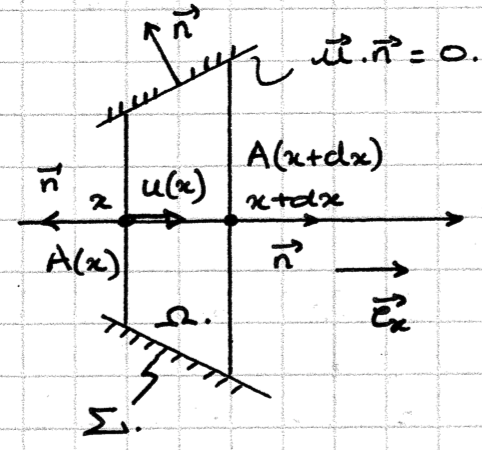
\includegraphics[width = 30mm]{volume_controle.png}}
	\end{picture}
\end{center}

%\bigskip \pause

\end{itemize}


\vspace{5mm}

\end{frame}

%-----------------------------------------------------------------------------------------

%-----------------------------------------------------------------------------------------
\begin{frame}{Bilan de masse}
%-----------------------------------------------------------------------------------------

\small

\begin{picture}(0, 0)(-70, 35)
	\put(0, 0){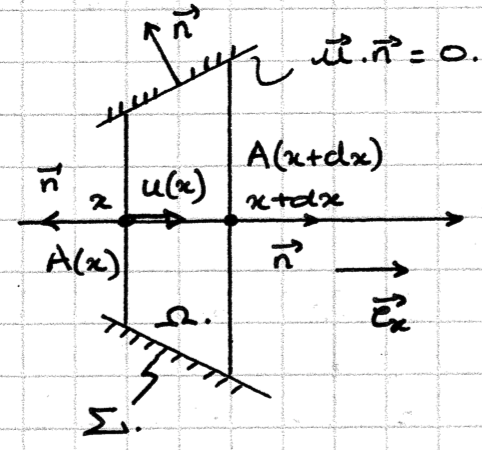
\includegraphics[width = 40mm]{volume_controle.png}}
\end{picture}

\begin{minipage}{60mm}
Bilan intégral de masse :
\[
	\color{blue}
	\dpdt{} \int_\Omega \rho \, dV = - \oint_{\partial \Omega} \rho \myvec{u} \cdot \myvec{n} \, dS
\]

\pause
%En omettant les barres, on en déduit \hfill \mbox{\color{gris} [Démonstration]}
%\[
%	A(x)\rho(x)u(x) = A(x+dx)\rho(x+dx) u(x+dx)
%\]

Soit, sous l'hypothèse monodimensionnelle :

$$
\color{red}	
\dot{m} = \rho_1 u_1 A_1 = \rho_2 u_2 A_2
$$ 

\pause
Ce qui s'écrit aussi sous forme différentielle :
\begin{equation}
	%\color{red}	\dot{m} \equiv \rho u A = Cte 
%	\quad \Leftrightarrow \quad
	\frac{d\rho}{\rho} + \frac{du}{u} + \frac{dA}{A} = 0
\end{equation}

\end{minipage}

\vspace{25mm}

\end{frame}

%-----------------------------------------------------------------------------------------
%\subsubsection{Bilan de quantité de mouvement}
%%-----------------------------------------------------------------------------------------
%\begin{frame}{Bilan de quantité de mouvement}
%%-----------------------------------------------------------------------------------------
%
%\small
%
%\begin{picture}(0, 0)(-75, 35)
%	\put(0, 0){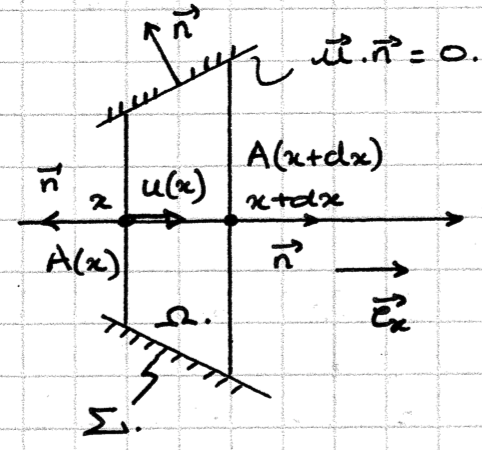
\includegraphics[width = 40mm]{volume_controle.png}}
%\end{picture}
%
%\begin{minipage}{65mm}
%Bilan intégral de quantité de mouvement :
%\[
%	\color{blue}
%	\dpdt{} \int_\Omega \rho \myvec{u} \, dV 
%	+ \oint_{ \Gamma_1 \cup \Gamma_2} [\rho \myvec{u} (\myvec{u} \cdot \myvec{n}) + p \myvec{n}] \, dS =
%	- \oint_{\Sigma} p\myvec{n} \, dS
%\]
%
%%%\pause
%%%En omettant les barres, on en déduit \hfill 
%%
%%Ce qui conduit au final à \mbox{\color{gris} [Démonstration]} :
%%\begin{eqnarray*}
%%	\rho(x) u^2(x) A(x) - \rho(x+dx) u^2(x+dx) A(x+dx) & &
%%	\\
%%	+ \; A(x) p(x) - A(x+dx) p(x+dx) & &
%%	\\
%%	- p(x) \left [ A(x) - A(x+dx) \right ] & = & 0
%%\end{eqnarray*}
%
%\pause
%
%\bigskip
%%Le débit massique $\rho u A = \dot{m}$ étant constant, on en déduit :
%
%Ce qui s'écrit aussi :
%
%\begin{eqnarray*}
%\left( \rho_2 u_2^2 +p_2 \right) A_2 - \left( \rho_1 u_1^2 +p_1 \right) A_1
%= \int_1^2 p(x) \frac{dA}{dx} dx
%%	\dot{m} \left [ u(x+dx) - u(x) \right ]
%%	+ A(x+dx) \left [ p(x+dx) - p(x)\right ] & = & 0
%\end{eqnarray*}
%
%\end{minipage}
%
%%\pause
%
%\bigskip
%
%\bigskip
%
%
%Dans la limite $dx\rightarrow 0$, on obtient donc :
%\[
%	\dot{m} \, du + A dp = 0 \quad \Leftrightarrow \quad \rho u A \, du + A dp = 0
%\]
%
%soit encore :
%\begin{equation}
%	\color{red}
%	\rho u du + dp = 0
%\end{equation}
%
%%\vspace{5mm}
%
%\end{frame}
%
%%-----------------------------------------------------------------------------------------
%%\subsubsection{Bilan d'énergie totale}
%%-----------------------------------------------------------------------------------------
%\begin{frame}{Bilan d'énergie totale}
%%-----------------------------------------------------------------------------------------
%
%\small
%
%En notant $\color{vert} e+u^2/2$ l'\textcolor{vert}{énergie totale} 
%par unité de masse, où $u^2 = ||\myvec{u}||^2$,
%le premier principe \\
%de la thermodynamique appliqué au système ouvert constitué
%du fluide contenu dans le volume \\ de contrôle fixe $\Omega$ s'écrit : \pause
%
%\[
%	\color{blue}
%	\dpdt{} \int_\Omega \rho \left ( e+\frac{1}{2} u^2 \right ) \, dV 
%	= 
%	- \oint_{\partial \Omega} \rho \left ( e+\frac{1}{2} u^2 \right ) \myvec{u} \cdot \myvec{n} \, dS
%	+ \mathcal{P}_{m, ext}
%	+ \mathcal{P}_{th, ext}
%\]
%\pause
%
%où la puissance mécanique des efforts extérieurs se réduit à
%\[
%	\mathcal{P}_{m, ext} = \oint_{\partial \Omega} \left(-p \myvec{n}\ \right ) \cdot \myvec{u} \, dS
%\]
%\pause
%et l'absence d'échange de chaleur avec l'extérieur (hypothèse adiabatique) implique
%\[
%	\mathcal{P}_{th, ext} = 0
%\]
%
%\pause
%\bigskip
%
%Le bilan intégral d'énergie totale a donc pour expression 
%\[
%	\oint_{\partial \Omega} \rho \left ( e+\frac{1}{2} u^2 + \frac{p}{\rho}\right ) \myvec{u} \cdot \myvec{n} \, dS = 0
%\]
%
%En appliquant les mêmes étapes de calcul que pour le bilan de masse, on obtient \textcolor{vert}{(exercice)} :
%\begin{equation*}
%	\rho \left( e+ \frac{p}{\rho} +\frac{1}{2} u^2 \right ) u A = Cte
%	\quad \Rightarrow \quad
%	\color{red} e+ \frac{p}{\rho}+\frac{1}{2} u^2  = Cte
%	\quad \mbox{\color{black} (car $\dot{m} = \rho u A = Cte$)}
%\end{equation*}
%
%\vspace{0mm}
%
%\end{frame}
%
%%-----------------------------------------------------------------------------------------
%\begin{frame}{Bilan d'enthalpie}
%%-----------------------------------------------------------------------------------------
%
%\small
%
%Le bilan d'énergie totale
%peut se réécrire de manière équivalente en introduisant l'\textcolor{vert}{enthalpie spécifique} 
%moyenne
%\[
%	\color{vert}
%	h \equiv e + \frac{p}{\rho} = c_p \, T
%\]
%où $c_p$ désigne la capacité calorifique massique à pression constante du gaz parfait.
%
%\medskip \pause 
%
%On déduit alors du bilan d'énergie totale le bilan pour l'enthalpie spécifique :
%\[
%	e+\frac{1}{2} u^2 + \frac{p}{\rho} = Cte \; \Leftrightarrow \; h + \frac{1}{2} u^2 = Cte 
%\]
%\begin{equation} 
%	\Leftrightarrow \; \color{red}
%	dh + u \, du = 0 
%	\quad \mbox{\color{black} ou encore} \quad
%	c_p dT + u\, du = 0
%\end{equation}
%
%\medskip \pause
%
%On peut aussi introduire l'\textcolor{vert}{enthalpie totale} moyenne, somme de l'énergie "thermodynamique" 
%(enthalpie spécifique) et de l'énergie cinétique :
%\[
%	\color{vert}
%	{\cal H} \equiv h + \frac{1}{2} u^2 = e + \frac{p}{\rho} + \frac{1}{2} u^2 = c_p \, T + \frac{1}{2} u^2
%\]
%\pause
%Le bilan pour l'enthalpie totale s'écrit alors :
%\[
%	\color{red}
%  d{\cal H}  = 0 \quad \Leftrightarrow \quad {\cal H} = Cte
%\]
%L'enthalpie totale est donc conservée.
%
%\vspace{0mm}
%
%\end{frame}
%

\begin{frame}{Bilans d'énergie et d'entropie }
\small

\begin{itemize}

\item Comme vu précédemment, {\bf la conservation de l'énergie totale}, se met sous la forme 
 (en considérant une ligne de courant traversant les sections 1 et 2) :

$$
h_1  + \frac{u_1^2}{2} = h_2  + \frac{u_2^2}{2}
$$



\pause
\bigskip

Sous forme différentielle, ceci se met également sous la forme 
$$
 dh + u du = 0 \qquad { ou encore } (\gamma -1) 2c dc + u du = 0.
$$  

Ce qui peut s'écrire également (démonstration) :


$$\color{red}\frac{dT}{T}  = - \frac{M^2}{\gamma - 1} \frac{du}{u} = 0.$$
%\end{frame}


%\begin{frame}{Bilan d'entropie}
%\small
\item 
L'écoulement étant isentropique, le {\bf bilan d'entropie}  est équivalent à l'{\bf équation de Laplace } sous l'une ou l'autre de ses formes :

$$
T_1 \rho_1^{1-\gamma} =   T_2 \rho_2^{1-\gamma}
$$


\pause
\bigskip

Sous forme différentielle, ceci se met également sous la forme 
$$
\color{red} \frac{dT}{T} +  (1- \gamma) \frac{d\rho}{\rho}  = 0
$$  

\end{itemize}

\end{frame}


%
%%-----------------------------------------------------------------------------------------
%\subsubsection{Bilan d'entropie}
%%-----------------------------------------------------------------------------------------
%\begin{frame}{Bilan d'entropie}
%%-----------------------------------------------------------------------------------------
%
%\small
%
%\textbf{Remarque :} le bilan d'entropie est contenu dans les bilans précédents.
%
%En effet 
%$$
%T ds = d h - \frac{1}{\rho} dp
%$$
%Ce qui, a partir des bilans de quantité de mouvement et d'enthalpie, conduit à  $\color{red} ds = 0$.
%
%\bigskip \pause
%
%On peut donc utiliser les relations de Laplace :
%
%%En effet, on peut vérifier que l'écoulement est isentropique :
%\[
%%	\mbox{\color{gris} [Démonstration] \; $\longrightarrow$ \;}
%	\color{red} 
%	T\rho^{1-\gamma} = Cte \quad \mbox{\color{black} et} \quad p\rho^{-\gamma} = Cte
%\]
%
%\medskip
%
%(NB : $\gamma = c_p/c_v = 1.4$ pour l'air)
%
%\vspace{20mm}
%
%\end{frame}

%-----------------------------------------------------------------------------------------
\begin{frame}{Récapitulatif}
%-----------------------------------------------------------------------------------------

\small

Les bilans de masse, d'énergie et d'entropie conduisent donc aux équations suivantes :

\begin{eqnarray}
	\rho u A = \dot{m} = Cte & \mbox{ou} & \color{red}\frac{d\rho}{\rho} + \frac{du}{u} + \frac{dA}{A} = 0
	\\
%	& & \color{red} \rho u \, du + dp = 0
%	\\
     {\cal H}  = h + \frac{1}{2}u^2 = c_p T + \frac{1}{2}u^2 = {\cal H}_i = Cte & \mbox{ou} & \color{red} \frac{dT}{T}  + \frac{M^2}{\gamma - 1} \frac{du}{u} = 0. 
     \\
     T \rho^{1-\gamma} = Cte & \mbox{ou} & \color{red} \color{red} \frac{dT}{T} +  (1- \gamma) \frac{d\rho}{\rho}  = 0.
     \end{eqnarray}

\bigskip

{\bf Remarque :} 

On n'a pas utilisé ici le bilan de quantité de mouvement .

Celui-ci se met sous la forme suivante 

$$ \rho u du + dp =0 $$

On peut  retrouver cette expression en combinant les bilans d'énergie et  d'entropie ainsi que l'équation d'état ({\em Exercice}).

%Le problème est a priori bien posé : il est décrit par 4 équations différentielles 
%pour les 4 inconnues cinématique $u(x)$
%et thermodynamiques $\rho(x)$, $p(x)$ et $T(x)$, qui dépendent de paramètres géométriques
%comme la loi de section $A(x)$ et de paramètres physiques tels le débit massique $\dot{m}$, 
%et les \textcolor{vert}{conditions génératrices}.

\vspace{10mm}

\end{frame}


%-----------------------------------------------------------------------------------------
%\subsubsection{Conditions génératrices}
%%-----------------------------------------------------------------------------------------
%\begin{frame}{Conditions génératrices}
%%-----------------------------------------------------------------------------------------
%
%\small
%
%\textbf{Définition :} \medskip
%
%on appelle conditions ou grandeurs \textcolor{vert}{génératrices} les valeurs prises 
%par les grandeurs thermodynamiques, notées $\rho_i$, $p_i$, $T_i$, au niveau d'un \textcolor{vert}{point d'arrêt}, \\ réel ou fictif, 
%c'est-à-dire à l'endroit où la vitesse de l'écoulement est nulle.
%
%\medskip
%
%Les grandeurs génératrices sont aussi appelées \textcolor{vert}{grandeurs d'arrêt}.
%
%\begin{center}
%	\begin{picture}(70, 25)(0, 0)
%		\put(0, 0){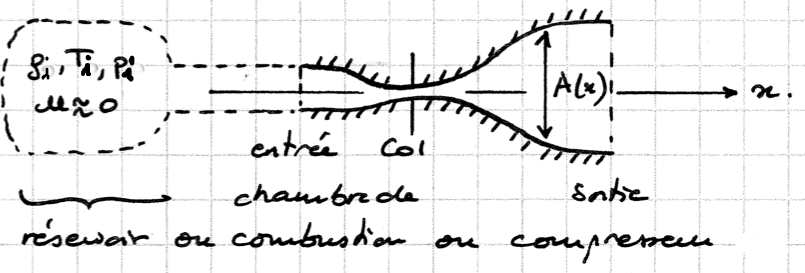
\includegraphics[width = 70mm]{conditions_generatrices.png}}
%	\end{picture}
%\end{center}
%
%Ces grandeurs sont en général connues ou fixées par les conditions opérationnelles \\ 
%(pression et température dans la chambre de combustion ou dans le compresseur \\
%en amont de la tuyère par exemple).
%
%
%\vspace{5mm}
%
%\end{frame}


%==========================================================================================
%\subsection{Résolution du problème}
%=========================================================================================


%-----------------------------------------------------------------------------------------
\subsubsection{Relation de Hugoniot}
%-----------------------------------------------------------------------------------------
\begin{frame}{Relation de Hugoniot}
%-----------------------------------------------------------------------------------------

\small

En combinant les bilans locaux de masse, énergie et entropie écrits précédemment, on démontre la relation de \textcolor{vert}{Hugoniot}
reliant les variations de vitesse dans une conduite de section variable $A(x)$ :
\[
	\mbox{\color{gris} [Démonstration] \; $\longrightarrow$ \;}
	\color{blue}
	\frac{du}{u}  =  -\frac{1}{1-M^2} \frac{dA}{A}
\]

On montre de même pour l'évolution de la pression : 
\[
	\mbox{\color{vert} [exercice] \; $\longrightarrow$ \;}
	\color{blue}
	\frac{dp}{p} = \gamma \frac{M^2}{1-M^2} \frac{dA}{A} 
\]

\pause

\textbf{Conséquences :} %\medskip 

%l'objectif est d'accélerer le fluide tout au long de la tuyère : \pause

\begin{itemize}
\item Pour un écoulement subsonique : 

Dans une section {\color{blue} convergente ($A \searrow $), alors $u \nearrow$} et $p \searrow$ (effet Venturi classique). 

Dans une section divergente ($A \nearrow $), alors $u \searrow$ et $p \nearrow$.
\pause
\medskip

\item Si l'écoulement est supersonique c'est l'inverse !

Dans une section convergente ($A \searrow $), alors $u \searrow$ et $p \nearrow$ 

Dans une section {\color{blue} divergente ($A \nearrow $), alors $u \nearrow$} et $p \searrow$.

\pause 
\medskip

%	à l'entrée de la tuyère l'écoulement est peu rapide $M<1$ \pause :
%	pour avoir accélération $du>0$, il faut $dA<0$ et donc un \textcolor{red}{convergent}
%	\pause
\item Pour accélérer l'écoulement tout le long de la tuyère il faut donc que celle-ci présente un {\color{blue} col} correspondant à un minimum de la section $A_c$. On a alors nécessairement \textcolor{red}{$M=1$ au col}.%($dA=0$).

%	l'écoulement accélère jusqu'à atteindre $M=1$ \pause :
%	pour continuer à accélérer $du>0$ l'écoulement pour $M>1$, il faut maintenant
%	$dA > 0$, donc un \textcolor{red}{divergent}

\pause 
\medskip

%\item
%\pause
	
\end{itemize}

Si ces conditions sont réunies on dit que \textcolor{red}{ la tuyère est amorcée.}

%On va voir que dans ce cas le débit de masse $\dot m$ est  imposé par la 
%\textcolor{blue}{dimension du col $A_c$} et  par les \textcolor{blue}{conditions génératrices.}


%\bigskip

%\pause

%\begin{center}
%	\begin{picture}(75, 25)(15, 0)
%		\put(0, 10){D'où la forme générique des tuyères :}
%		\put(45, 0){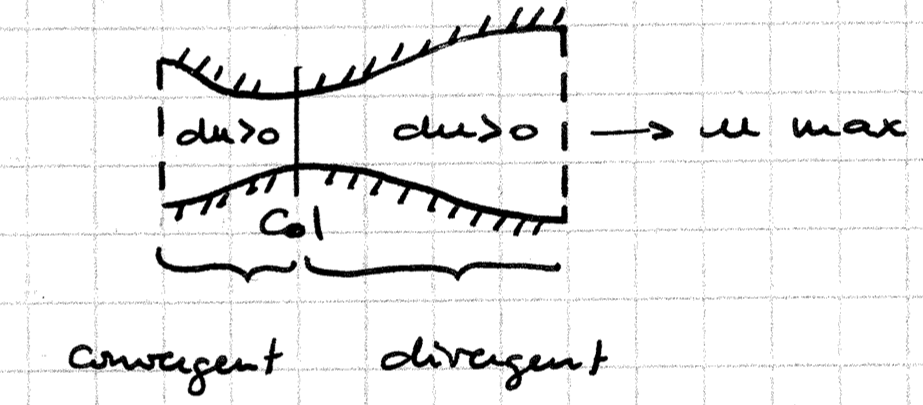
\includegraphics[width = 55mm]{Hugoniot.png}}
%	\end{picture}
%\end{center}


\vspace{0mm}

\end{frame}



%-----------------------------------------------------------------------------------------
%\subsubsection{Relations de Barré--St Venant}
%%-----------------------------------------------------------------------------------------
%\begin{frame}{Relations de Barré--St Venant}
%%-----------------------------------------------------------------------------------------
%
%\small
%
%\textbf{Objectif :} \medskip
%
%connaissant les conditions génératrices $\rho_0$, $p_0$, $T_0$ et la géométrie
%$A(x)$, est-il possible de déterminer l'évolution des grandeurs cinématique $u(x)$
%et thermodynamiques $\rho(x)$, $p(x)$ et $T(x)$ le long de la tuyère ?
%
%\begin{center}
%	\begin{picture}(70, 25)(0, 0)
%		\put(0, 0){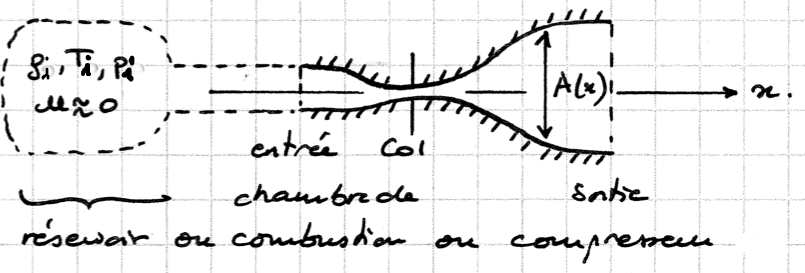
\includegraphics[width = 70mm]{conditions_generatrices.png}}
%	\end{picture}
%\end{center}
%
%\pause
%
%\textbf{Objectif intermédiaire:} \medskip
%
%on cherche d'abord à déterminer les relations dites de \textcolor{vert}{St--Venant}
%\[
%	\frac{T}{T_0}(M), \frac{\rho}{\rho_0}(M), \frac{p}{p_0}(M) \; \mbox{et} \; u(M)
%\]
%en fonction du nombre de Mach local $M = M(x)$, que l'on déterminera dans un deuxième temps.
%
%\vspace{5mm}
%
%\end{frame}

\subsubsection{Calcul de l'écoulement dans la tuyère}


%-----------------------------------------------------------------------------------------
\begin{frame}{Calcul de l'écoulement dans la tuyère}
%-----------------------------------------------------------------------------------------

\small

%\textbf{Bilan :} \medskip


%Pour terminer la résolution il faut maintenant calculer le débit de masse $\dot m$ en fonction des conditions génératrices, puis déterminer $M$ en fonction de $A$.


Revenons au calcul de l'écoulement dans la tuyère. 
\medskip 
\pause 

En supposant celle-ci {\bf amorcée},  on peut tout d'abord déduire le débit de masse
a partir des relations de Barré de St-Venant appliquées au col ($M=1$) :
\medskip
\pause 
$$
\color{red}
\dot m = {\dot m}_{amorce} = \rho_c u_c A_c = \beta \rho_i \sqrt{\gamma r T_i} A_c  \qquad \mbox{ avec } 
\beta = {\left(\frac{2}{\gamma+1}\right)}^{\frac{\gamma+1}{2(\gamma-1)}} \approx 0.5787
$$

\pause

On remarque que {\bf le débit de masse est entièrement fixé par la dimension du col et les conditions génératrices}
(indépendantes de la pression en sortie de tuyère  !)


\medskip

Pour pouvoir déterminer les conditions en tout point de la tuyère il reste maintenant à déterminer la relation entre $A$ et $M$.  
En écrivant $\dot m = \rho(M) u(M) A =  \rho_c u_c A_c$  on trouve \textcolor{green}{[exercice] :}

$$
\color{red}
\frac{A}{A_c} = \frac{\beta}{M}  {\left(1 + \frac{\gamma-1}{2}M^2 \right)}^{\frac{\gamma+1}{2(\gamma-1)}}
$$

Remarque : pour $A/A_c>1$ cette relation donne deux valeurs possibles de $M$, l'une subsonique (appliquable avant le col) et l'autre 
supersonique (appliquable après le col).


\medskip

\pause
Utilisation pratique :

Pour résoudre un problème on pourra utiliser les {\bf tables d'écoulements compressibles isentropiques} donnant 
$P/P_i, \rho/\rho_i, T/T_i, A/A_c$ en fonction de $M$.



\vspace{0mm}

\end{frame}


%-----------------------------------------------------------------------------------------
\begin{frame}{Exercice}
%-----------------------------------------------------------------------------------------

Exercice d'application (Chassaing, p. 249)

\medskip
Un réservoir contient de l'air sec à une pression $P_i= 10 Bars$, et une température de $T_i = 300K$.
Cet air s'écoule à travers une tuyère de section au col $A_c = 755 mm^3$ et de section de sortie $A_s = 1272 mm^2$.

\medskip


Calculez : $(a)$ les conditions (pression, température, masse volumique et vitesse) au col,
 $(b)$ le débit-masse,
 et $(c)$  les conditions en sortie.


\medskip 
$(d)$ mêmes questions pour une section de sortie $A_s = 1980 mm^2$. Les conditions de sortie sont-elles compatibles avec une sortie à l'air libre dans une atmosphère standard ?


 



\end{frame}

\subsection{Ondes de choc}

\subsubsection{Bilan sur le fonctionnement d'une tuyère (1)}

\begin{frame}{Bilan sur le fonctionnement d'une tuyère (1)}


\small
Considérons une tuyère de dimensions donnée (sections $A_c$ au col et $A_s$ en sortie). 

Récapitulons les écoulements possibles selon la valeur du rapport de détente $ P = p_i/p_{ext}$ :

\pause
\begin{itemize}

\item  Pour $p_i/p_{ext} = 1 $ :  Pas d'écoulement. 

 \pause 
\item Pour $1 < p_i/p_{ext} < P_1  $ : écoulement subsonique dans la totalité de la tuyère ($\dot m < {\dot m}_{amorce}$)

 \pause 
\item Pour $p_i/p_{ext} = P_1 $ : écoulement sonique au col ($\dot m = {\dot m}_{amorce}$) puis redevient subsonique 
 
 \pause 
\item Pour $p_i /p_{ext} = P_2$ : écoulement sonique au col ($\dot m = {\dot m}_{amorce}$)  puis supersonique dans le divergent.
(On parle de {\em tuyère adaptée}).

\end{itemize}
 
 \pause 
 \smallskip
 (Exercice : A l'aide des tables d'écoulement isentropique déterminez $P_1$ et $P_2$ dans le cas $A_s/A_c = 2$)
 
 
 
 
 {\bf Question :} que se passe-t-il pour d'autres valeurs possibles  du rapport de détente $ P = p_i/p_{ext}$ ?
 
\end{frame}

%-----------------------------------------------------------------------------------------
\begin{frame}{Régime discontinu d'une tuyère amorcée}
%-----------------------------------------------------------------------------------------

\small

%Remarque : l'hypothèse d'écoulement isentropique amorcé dans une tuyère impose
%une pression $p_s$ en sortie de la tuyère ($A=A_s$).

Si $P_1< p_s / p_{ext} <  P_2$ La pression doit nécessairement remonter pour s'adapter aux conditions rencontrées en sortie de tuyère .

La seule manière est de le faire de manière brutale (non isentropique) a travers une {\color{rouge} Onde de choc}.


\medskip

\pause


\begin{picture}(120, 63)
	\put(2, 35){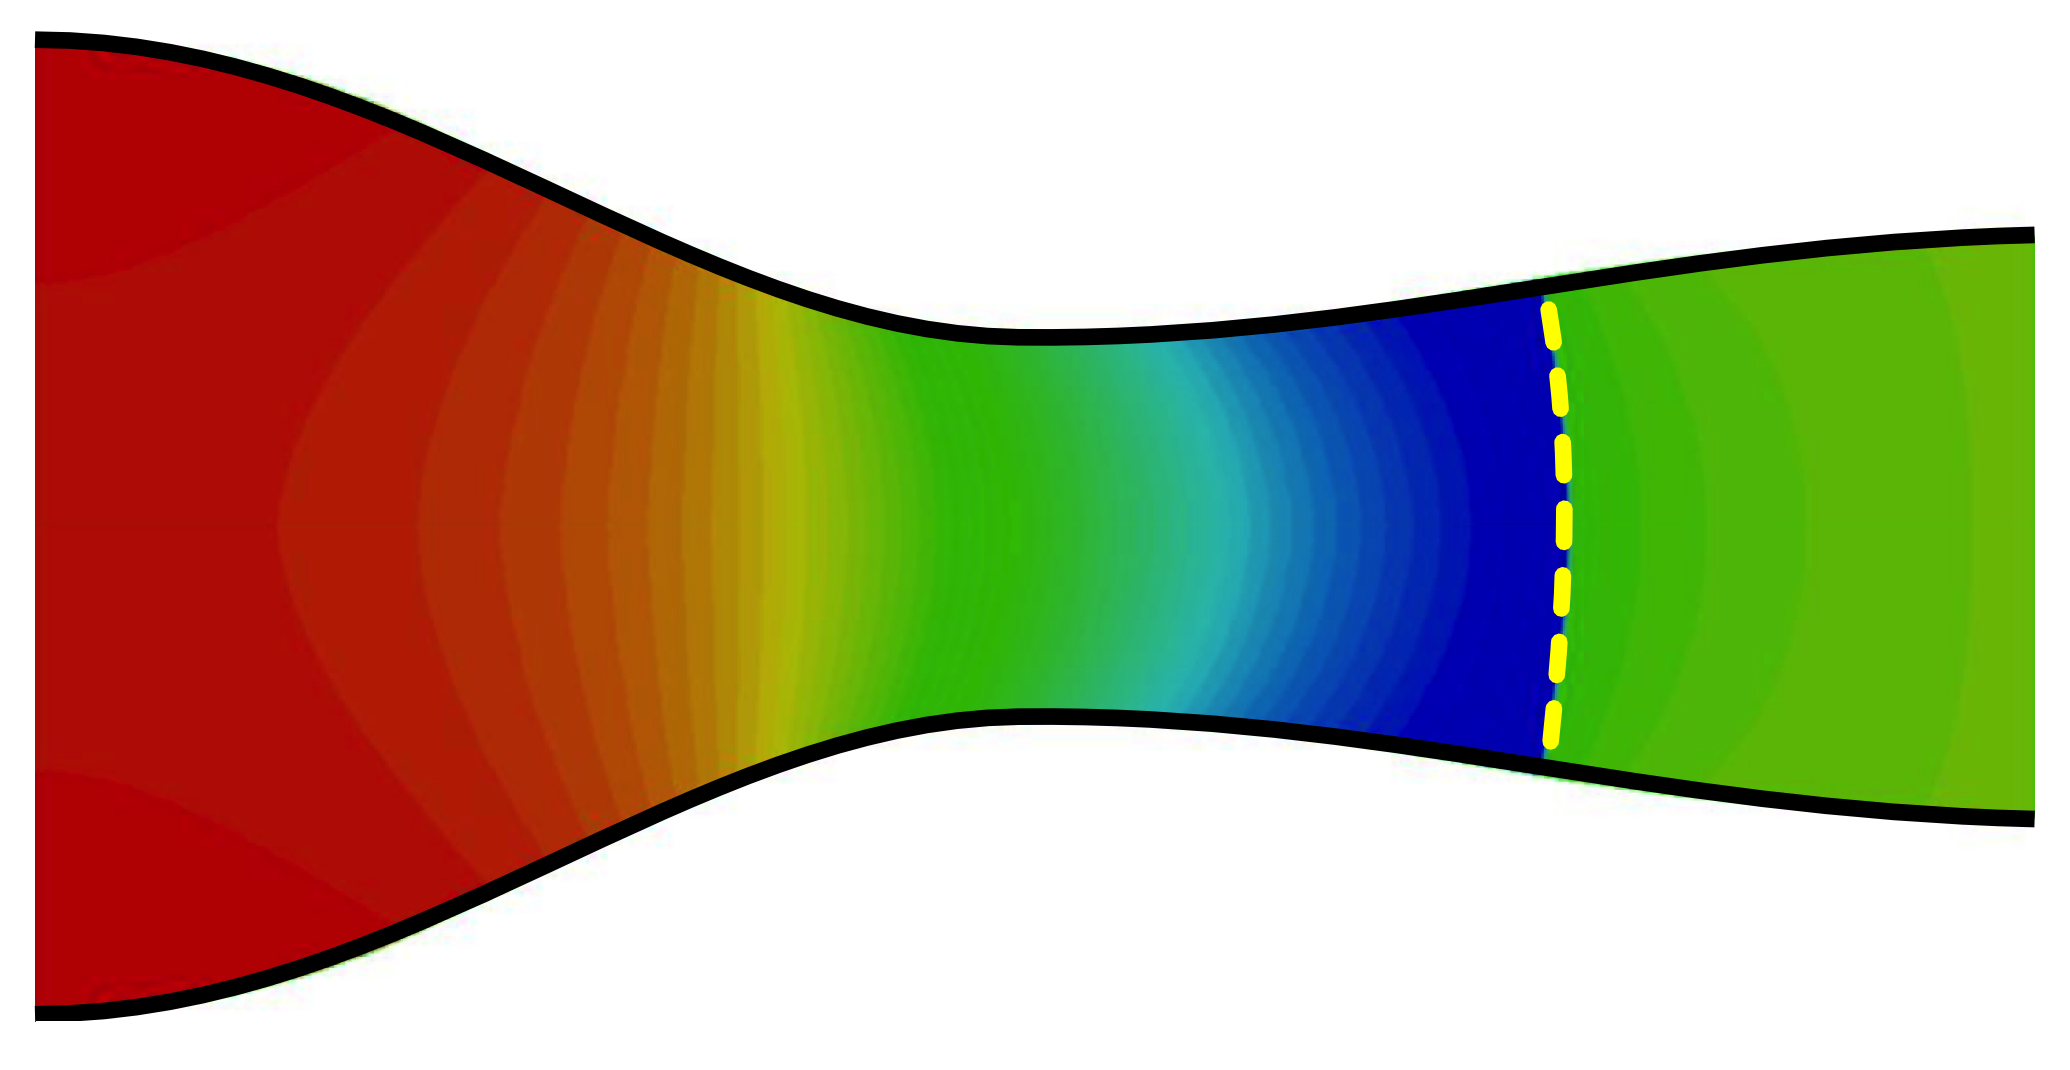
\includegraphics[width=50mm]{Nozzle/pressurein_nozzle.png}}
	\put(55, 40){
\includegraphics[height=16mm, width=3mm]{Nozzle/colorbar.png}}
	\put(0, 18){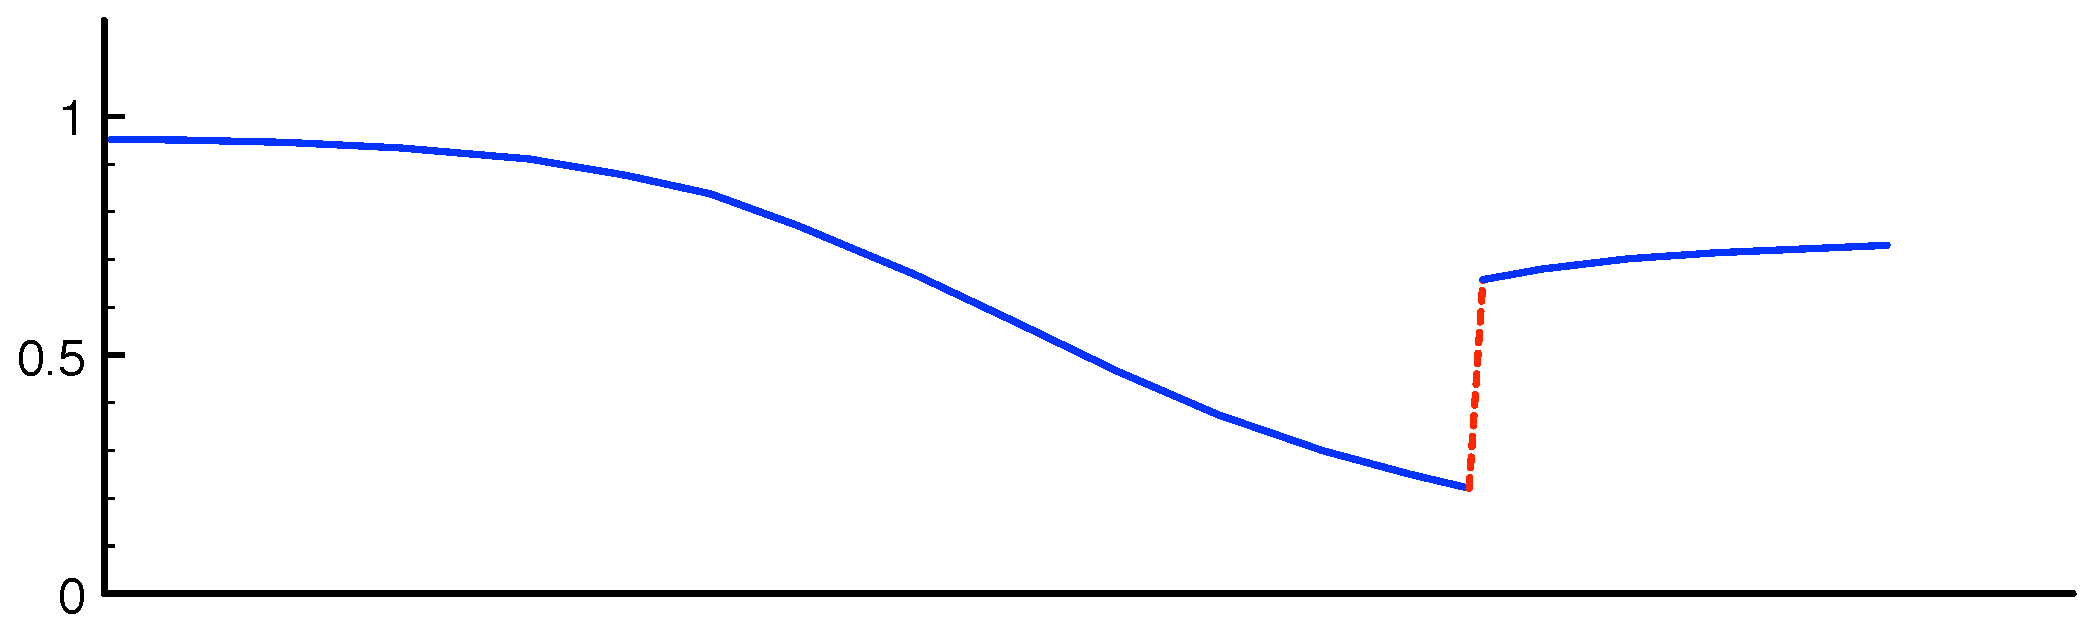
\includegraphics[width=55mm]{Nozzle/pressure.pdf}}
	\put(0, 0){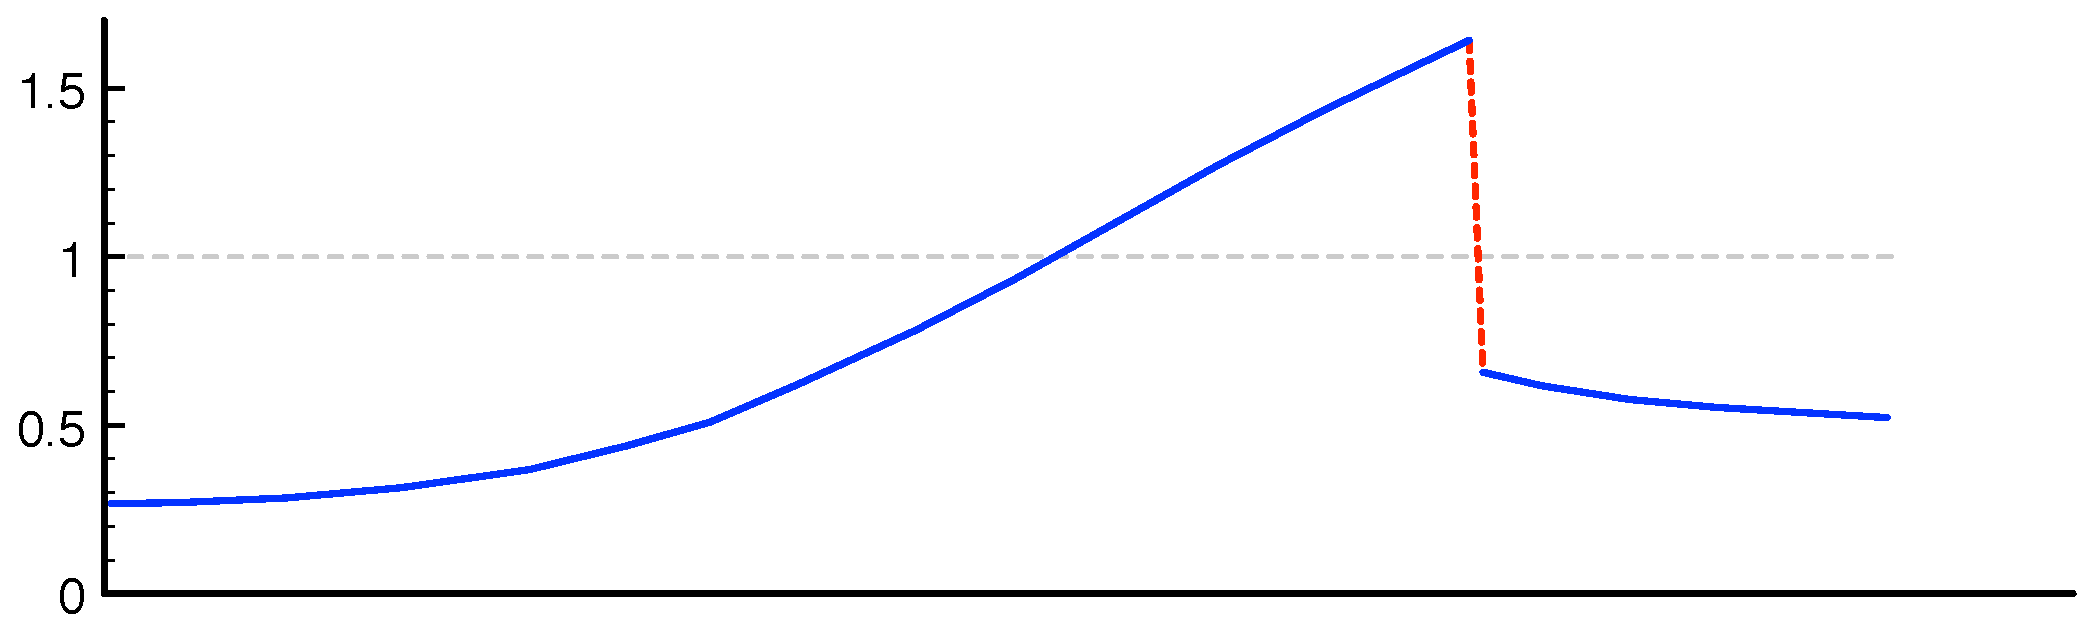
\includegraphics[width=55mm]{Nozzle/Mach_nozzle.pdf}}
	\put(27.7, 0){\color{vert}\line(0, 1){54}}
	\put(4, 48.2){\color{yellow}\vector(1, 0){5}}
	\put(25, 38){\colorbox{white}{\color{vert}col}}
	\put(54, 58){$p/p_i$}
	\put(10, 61){champ de pression dans la tuyère}
	\put(15, 58){(simulation Fluent \copyright)}
	\put(4, 25){$p/p_i$}
	\put(4, 7){$M$}
	\put(39.2, 36.5){\color{rouge} \vector(0, 1){5}}
	\put(39.2, 32.7){\color{rouge} \vector(0, -1){5}}
	\put(52.2, 32.2){\color{vert} $p_{\mbox{\scriptsize ext}}/p_i$}
	\put(55.2, 28.1){\color{vert} \line(0, 1){3}}
	\put(55.2, 28.1){\color{vert} \vector(-1, 0){5}}
	\put(36, 34){\color{rouge} \bf CHOC}
	\put(66, 32){\begin{minipage}{40mm}
									%Si la pression en sortie de tuyère 
									%n'est pas adaptée à la pression extérieure
									
									\medskip
							 		$\rightarrow$ existence d'un choc d'adaptation 
									\mytabbing{$\rightarrow$} dans le divergent 
									
									\medskip
									$\rightarrow$ après le choc, l'écoulement 
									\mytabbing{$\rightarrow$} redevient subsonique et décélère
									\mytabbing{$\rightarrow$} (cf. relation d'Hugoniot)
									
									\bigskip
									
									Ce régime de fonctionnement est donc à éviter puisqu'il ne permet 
									pas d'accélérer continûment l'écoulement jusqu'en sortie de tuyère.
									
									\bigskip
									Il n'est alors pas possible d'obtenir une poussée optimale.
					    \end{minipage}}
\end{picture}


{\bf Remarque :} pour des rapports de détente élevés on peut également avoir un {\bf choc oblique } en sortie de tuyère.
(Illustrations : programme {\sc nozzleGUI.m }).

\vspace{0mm}

\end{frame}


%%%%%%%%%%%%%%%%%%%%%%%%%%%%%%%%%%%%%%%%%%%%%%%%%%%%%%%%

\begin{frame}{Introduction aux ondes de choc : une analogie}

\small

Analogie automobile :
 \smallskip
Considérons un automobiliste roulant à la vitesse $U$ et notons  $L$ la distance le séparant de l'automobiliste précédent.

 \smallskip
Que se passe-t-il si l'automobiliste précédent freine  ???

 \pause 
 \smallskip

\begin{itemize}
\item Vitesse de l'automobiliste : $U$

\item Vitesse de l'information "il faut freiner" dans le référentiel du conducteur : $c = L/\tau$ ($\tau$ temps de réaction du conducteur ; $\approx 1 s$)

\item Vitesse de l'information "il faut freiner" dans le référentiel fixe : $U-c$.

\end{itemize}

Deux possibilités :

\begin{itemize}
\item Si $U-c<0$ : l'information remonte la file de voiture. Les conducteurs ont le temps d'adapter leur conduite.

$=>$ Circulation fluide 

\pause
\item Si $U-c>0$ : les automobiles n'ont pas le temps de s'adapter, ils freinent brutalement !

$=>$ Bouchon ! (ou pire...)

\end{itemize}

\pause


Revenons au cas de la tuyère. Comment le fluide s'adapte-t-il à une pression imposée en sortie de tuyère ?
\pause
\begin{itemize}
\item Si $u<c$ ( ou $M = u/c <1$ ) : l'information "la sortie nécessite une adaptation" peut remonter l'écoulement. Celui-ci s'adapte.
\pause
\item Si $U>c$ ( ou $M = U/c >1$ ) :  l'information "la sortie nécessite une adaptation" ne peut remonter l'écoulement.
\pause
$=>$ Choc

\end{itemize}
\end{frame}

%%%%%%%%%%%%%%%%%%%%%%%%%%%%%%%%%%%%%%%%%%%%%%%%%%%%%%%%%
%-----------------------------------------------------------------------------------------
\subsubsection{Calcul des conditions de choc}
%-----------------------------------------------------------------------------------------
\begin{frame}{Calcul des conditions de choc : 1 écriture des équations-bilan}
%-----------------------------------------------------------------------------------------

\small

Soit le volume de contrôle fixe infinitésimal $\Omega$, de normale sortante $\myvec{n}$,
suivant :

\begin{center}
	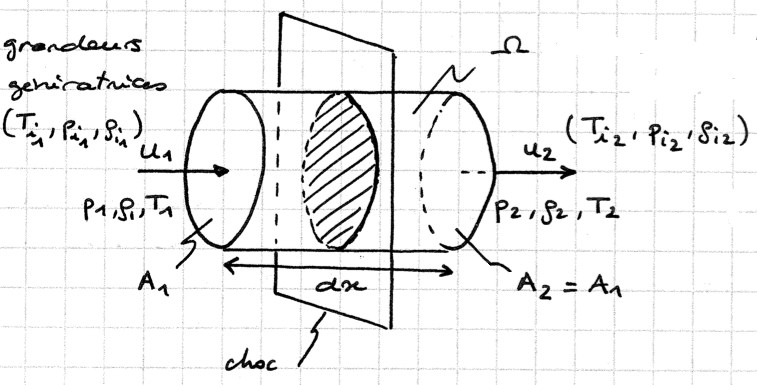
\includegraphics[width=70mm]{volume_controle_choc.png}
\end{center}

On notera par l'indice 1 toute quantité physique \textsl{juste avant le choc} (amont), et
\mytabbing{On notera} par l'indice 2 toute quantité physique \textsl{juste après le choc} (aval).

\vspace{5mm}

\pause 
Les bilans de masse, quantité de mouvement et énergie s'écrivent alors respectivement :

\begin{equation}
	\color{rouge}
	\rho_1 u_1 = \rho_2 u_2
\end{equation}
\begin{equation}
	\color{rouge}
	p_1 + \rho_1 u_1^2 = p_2+\rho_2 u_2^2
\end{equation}
\begin{equation}
	\color{rouge}
	C_p T_1 + \frac{u_1^2}{2} = C_p T_2 + \frac{u_2^2}{2}
\end{equation}

\end{frame}

\begin{frame}{Calcul des conditions de choc : 2 résolution}
\small

En notant $M_1 = u_1/c_1$ et $M_2 = u_2/c_2$ les nombres de Mach juste avant et juste après le choc,

la résolution du problème (exercice complémentaire) conduit à :

\begin{equation}
	\color{rouge}
	M_2^2 = \frac{2+(\gamma-1)M_1^2}{2\gamma M_1^2 +1-\gamma}
\end{equation}


\begin{eqnarray}
	\color{rouge} \frac{T_2}{T_1}(M_1) 
	& 
	\color{rouge} = 
	& 
	\color{rouge} \frac{2 + (\gamma-1)M_1^2}{(\gamma+1)^2M_1^2}\left ( 2\gamma M_1^2 + 1 -\gamma\right )
	\\
	\color{rouge} \frac{p_2}{p_1}(M_1) 
	& 
	\color{rouge} = 
	& 
	\color{rouge} 1 + \frac{2\gamma}{\gamma+1}\left ( M_1^2 - 1\right )
	\\
	\color{rouge} \frac{\rho_2}{\rho_1} (M_1) 
	& 
	\color{rouge} = 
	& 
	\color{rouge} \frac{(\gamma+1) M_1^2}{2+(\gamma-1)M_1^2} \quad = \quad \frac{u_1}{u_2}(M_1)
	\end{eqnarray}


{\bf Remarque : } ces relations peuvent se combiner pour obtenir le saut d'entropie a travers le choc :

\begin{eqnarray}
\color{rouge} \frac{\left[ s_2- s_1  \right]}{c_v}
& \color{rouge} = 
&
	\color{rouge}  \ln \left[ \frac{p_2}{p_1} \left( \frac{\rho_2}{\rho_1}\right)^{-\gamma} \right]
	\\
& \color{rouge} = & \color{rouge} \ln (1 + \beta) + \gamma \ln \left( 1+\frac{\gamma-1}{2 \gamma} \beta \right) 
- \gamma \ln \left( 1+\frac{\gamma+1}{2 \gamma} \beta \right)
\mbox{ avec } \beta = p_2/p_1-1 \nonumber
	\end{eqnarray}

On vérifie que $s_2-s_1>0$ si $M_1>1$ ; on a alors $M_2<1$. 

\end{frame}



\subsubsection{Bilan sur le fonctionnement d'une tuyère (2)}

\begin{frame}{Bilan sur le fonctionnement d'une tuyère (2)}


\small

On peut donc compléter la liste des écoulements possibles selon la valeur du rapport de détente $ P = p_i/p_{ext}$ :

\pause
\begin{itemize}

\item  Pour $p_i/p_{ext} = 1 $ :  Pas d'écoulement. 

\item Pour $1 < p_i/p_{ext} < P_1  $ : écoulement subsonique dans la totalité de la tuyère ($\dot m < {\dot m}_{amorce}$)

\item Pour $p_i/p_{ext} = P_1 $ : écoulement sonique au col ($\dot m = {\dot m}_{amorce}$) puis redevient subsonique 
 
 \item Pour $P_1<p_i /p_{ext} < P_2 $ : écoulement sonique au col ($\dot m = {\dot m}_{amorce}$)  puis supersonique, 
{\color{rouge}  puis choc}, puis l'écoulement redevient subsonique 
 
\item Pour $p_i /p_{ext} = P_2 $ : écoulement sonique au col ($\dot m = {\dot m}_{amorce}$)  puis supersonique dans le divergent.
(On parle de {\em tuyère adaptée}).

\item Pour $p_i /p_{ext} > P_2 $ : écoulement sonique au col ($\dot m = {\dot m}_{amorce}$)  puis supersonique dans le divergent, 
puis formation d'une onde de détente en sortie (écoulement surdétendu).


\end{itemize}
 
 On peut montrer que parmi tous ces cas celui permettant de maximiser la poussée est le cas adapté.

\end{frame}

%\begin{frame}{Complément : estimation de l'épaissseur d'une onde de choc} 

%Cherchons à estimer l'épaisseur d'une onde de choc $\delta$ à l'aide du bilan local d'entropie.

%Supposons que l'approche milieu continu reste valable à l'intérieur du choc.





%Supposons que la dissipation se 





%
%\medskip
%
%$\rightarrow$ conservation du débit massique $\rho u A = \dot{m}$ :
%
%\medskip
%
%\pause 
%
%Si on suppose connu $\rho(M) u(M) A(x) = \dot{m}$, alors
%\[
%	\dot{m} = \rho_0 \sqrt{\gamma r T_0} A(x) \times g(M)
%\] 
%avec (exercice) :
%\[
%	g(M) = M \left ( 1 + \frac{\gamma - 1}{2} M^2 \right )^{\dfrac{\gamma +1}{2(\gamma-1)}}
%	\pause
%	= \frac{\dot{m}}{\rho_0 \sqrt{\gamma r T_0} A(x)} = f(x) \; \mbox{fonction de $x$ donnée}
%\]
%
%\pause
%\begin{center}
%	\begin{picture}(65, 20)(0, 0)
%		\put(0, 0){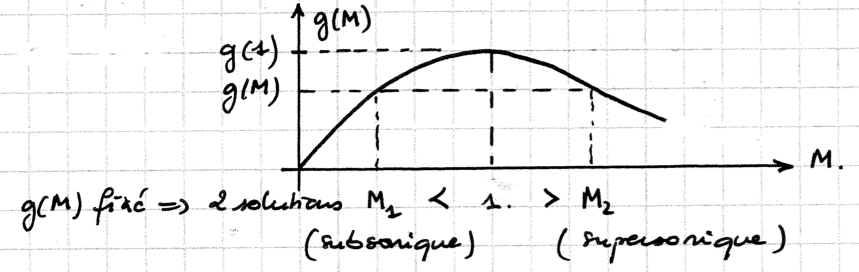
\includegraphics[width = 65mm]{fonction_g.png}}
%	\end{picture}
%\end{center}
%
%\pause
%D'où $f(x)$ connue $\Rightarrow$ $g(M)$ connue $\Rightarrow$ $M(x)$ connu en fonction des données du problème.


% \begin{frame}
%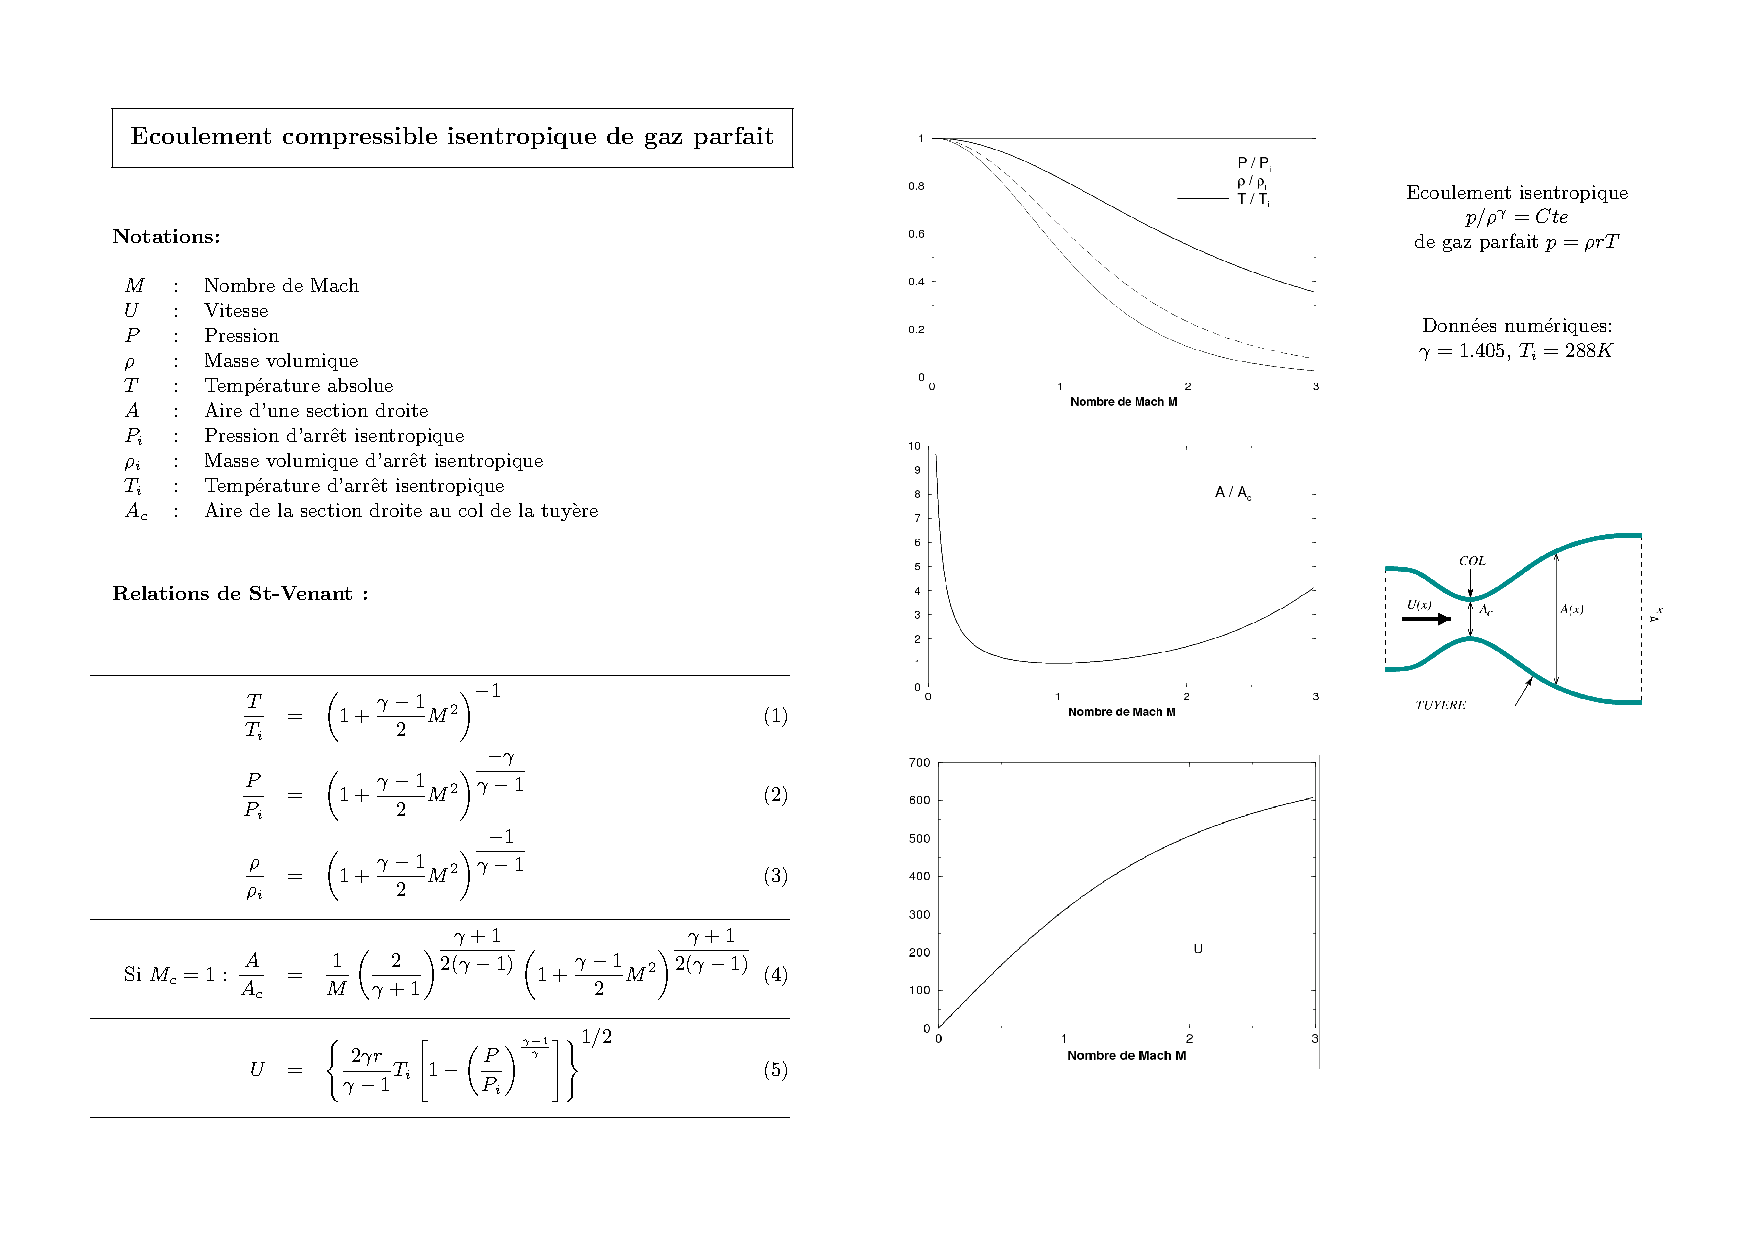
\includepdf[pages=1-2, landscape]{Figures/St_Venant.pdf}
%\end{frame}

%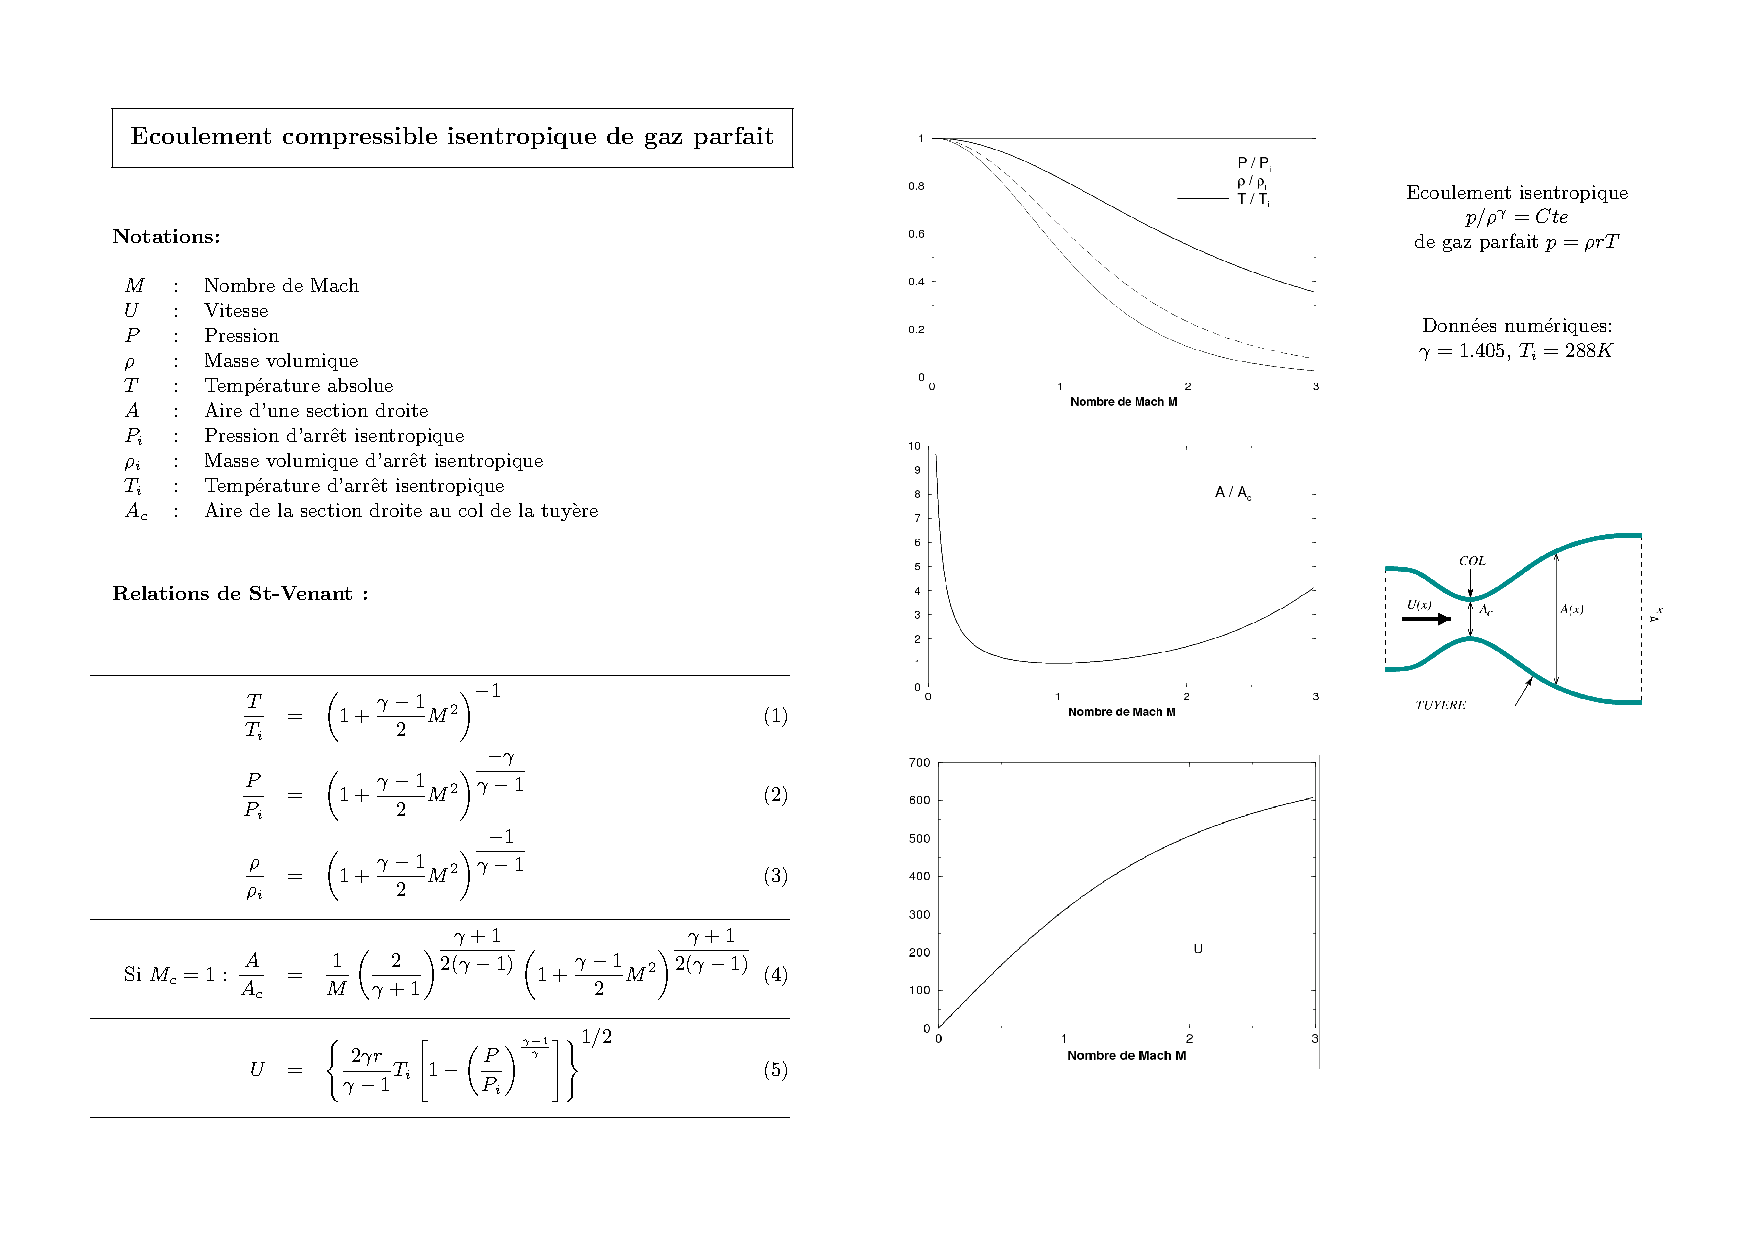
\includegraphics[pages=1-2,width=\linewidth]{Figures/St_Venant.pdf}



